%%%%%%%%%%%%%%%%%%%%%%%%%%%%%%%%%%%%%%%%%%%%%%%%%%%%%%%%%%%%%%%%%%%%%%%%%%%%%%%%
%%%%%%%%%%%%%%%%%%%%  Set document class, and configure it  %%%%%%%%%%%%%%%%%%%%
%%%%%%%%%%%%%%%%%%%%%%%%%%%%%%%%%%%%%%%%%%%%%%%%%%%%%%%%%%%%%%%%%%%%%%%%%%%%%%%%


% For a current list of options, see:
% `Define options for every class' and `Justification options for margin notes' sections in the `tufte-common.def' file
% This should provide you with the most accurate and up-to-date list of options as that's where they are defined
% Alternatively compile this document with the `debug' and search log output for: `Tufte-LaTeX settings'
% This sample book should also contain current list of options with explanation in the `Document Class Options' section
\documentclass[a4paper]{tufte-book}

% If you wish to add text to blank pages from \cleardoublepage command, uncomment this block and add your text:
%
% \renewcommand*{\blankpagetext}{
%   This page intentionally contains only this sentence.
% }

% Used for generating the index at the end of the document
\usepackage{makeidx}
\makeindex

% Used for adding images/graphics to the document
\usepackage{graphicx}
  % Set default scaling for included graphics
  \setkeys{Gin}{width=\linewidth,totalheight=\textheight,keepaspectratio}
  % Define base path for graphics, change this as needed
  \graphicspath{{graphics/}}

% Improves the quality of tables in LaTeX
% It provides useful commands, and ads some behind the scenes optimizations
% Tables created by this package are similar to the tables in Tufte's books
\usepackage{booktabs}

% Provides a way to set units in typographically correct way
% It includes the `nicefrac' package to provide nicer looking fractions
% Common commands include \unit[<value>]{<unit>}, \nicefrac{<num>}{<den>}, and \unitfrac[<value>]{<num>}{<den>}
% The \nicefrac can take a font command as an optional argument
\usepackage{units}

% Extends verbatim with new environments, and more features
\usepackage{fancyvrb}
  % Sets default verbatim font, smaller than default
  \fvset{fontsize=\small}

% Changes how the date is displayed in the document, and provides extra date related commands
% I prefer the ISO format yyyy-mm-dd, but it can be changed as needed
% Also used to print <month> <year> in the copyright page
\usepackage[style=iso,en-US]{datetime2}

% Can enable or disable hyphenation of words, even in TT font environments
\usepackage[htt]{hyphenat}

% Used for extra cross-referencing commands
\usepackage[noabbrev,nameinlink]{cleveref}


%%%%%%%%%%%%%%%%%%%%%%%%%%%%%%%%%%%%%%%%%%%%%%%%%%%%%%%%%%%%%%%%%%%%%%%%%%%%%%%%
%%  Define document metadata, and other useful things like bibliography file  %%
%%%%%%%%%%%%%%%%%%%%%%%%%%%%%%%%%%%%%%%%%%%%%%%%%%%%%%%%%%%%%%%%%%%%%%%%%%%%%%%%


\title{A Tufte-Style Book\thanks{Thanks to Edward R.~Tufte for his inspiration.}}
\author[The Tufte-LaTeX Developers]{The Tufte-LaTeX\ Developers}
\publisher{MJ Publishing House}
%\date{2025-01-28} % If the \date command is omitted, current date will be used instead

% Debugging
%\geometry{showframe} % display margins for debugging page layout

% Define BibLaTeX resource file
\addbibresource{sample-bibliography.bib}


%%%%%%%%%%%%%%%%%%%%%%%%%%%%%%%%%%%%%%%%%%%%%%%%%%%%%%%%%%%%%%%%%%%%%%%%%%%%%%%%
%%%%%%  These can be removed in actual documents, only used for examples  %%%%%%
%%%%%%%%%%%%%%%%%%%%%%%%%%%%%%%%%%%%%%%%%%%%%%%%%%%%%%%%%%%%%%%%%%%%%%%%%%%%%%%%


% Generates dummy text used in examples, sets the language to use for hyphenation rules
\usepackage[language=english]{lipsum}

% Tries to intuit whether or not to add a space after a command
% Used in some documentation commands here, but can be used in other places as well
\usepackage{xspace}

% Provides commands to print out nicely formatted LaTeX logos in text
\usepackage{hologo}

% Prints argument within hanging parentheses (i.e., parentheses that take up no horizontal space)
% Useful in tables where space is at a premium
\newcommand{\hangp}[1]{\makebox[0pt][r]{(}#1\makebox[0pt][l]{)}}

% Prints an asterisk that takes up no horizontal space, also useful in tables
\newcommand{\hangstar}{\makebox[0pt][l]{*}}

% Shortcuts for printing Tufte's book titles
% The lowercase commands will produce the initials of the book title in italics
% The all-caps commands will print out the full title of the book in italics
% Uses xspace to add a space after the command unless it's followed by punctuation
\newcommand{\vdqi}{\textit{VDQI}\xspace}
\newcommand{\ei}{\textit{EI}\xspace}
\newcommand{\ve}{\textit{VE}\xspace}
\newcommand{\be}{\textit{BE}\xspace}
\newcommand{\VDQI}{\textit{The Visual Display of Quantitative Information}\xspace}
\newcommand{\EI}{\textit{Envisioning Information}\xspace}
\newcommand{\VE}{\textit{Visual Explanations}\xspace}
\newcommand{\BE}{\textit{Beautiful Evidence}\xspace}

% Shortcut for printing the Tufte-LaTeX class name
\newcommand{\TL}{Tufte-\hologo{LaTeX}\xspace}

% Shortcut for printing month's name (e.g., January) and then the year (e.g., 2008)
% Based on current date, used on the copyright page to mark the first printing date
\makeatletter
  \newcommand{\monthAndYear}{\DTMenglishmonthname{\@dtm@month} \@dtm@year}
\makeatother
% For some reason XeLaTeX does not recognize the `\@dtm@month' and `\@dtm@year' commands
% Therefore it needs a different command to print the month and year
% If you're not using XeLaTeX, you can remove this block
\makeatletter
  \ifxetex%
    \renewcommand{\monthAndYear}{%
      \ifcase\month%
        \or\ January%
        \or\ February%
        \or\ March%
        \or\ April%
        \or\ May%
        \or\ June%
        \or\ July%
        \or\ August%
        \or\ September%
        \or\ October%
        \or\ November%
        \or\ December%
      \fi\space\number\year%
    }
  \fi
\makeatother


% Shortcut for printing of an epigraph, used on the first page of the book
% Prints an epigraph and speaker in all-caps, double-space type, sans or serif
\newcommand{\openepigraph}[2]{%
  \begin{fullwidth}
    % Set font based on sftitle option, either sans or serif
    \ifthenelse{\boolean{@tufte@sftitle}}{%
      \sffamily\large%
    }{%
      \rmfamily\large%
    }%
    % Print epigraph and speaker, #1 epigraph, #2 speaker
    \begin{doublespace}
      \noindent\allcaps{#1}\\
      \noindent\allcaps{#2}
    \end{doublespace}
  \end{fullwidth}
}

% Inserts a blank page with an `empty' page style (no folios, heads, or footers)
\newcommand{\blankpage}{\newpage\hbox{}\thispagestyle{empty}\newpage}

% Typesets the font size, leading, and measure in the form of 10/12x26 pc.
\newcommand{\measure}[3]{#1/#2\( \times \)\unit[#3]{pc}}

% Shortcuts for typesetting the documentation
% Highlights text in tufte-orange color
\newcommand{\hlorange}[1]{\textcolor{tufte-orange}{#1}}
% Creates a box wide enough to contain the text, positioning it to the right
\newcommand{\hangleft}[1]{\makebox[0pt][r]{#1}}
% Hairspace adds a tiny (less that 0.4mm wide) space between characters
\newcommand{\hairsp}{\hspace{1pt}}
% Halfquad adds a space equal to half a quad space (that's a space in current font size)
\newcommand{\hquad}{\hspace{.5em}}
% Prints an em-dash in the text, used in tables for N/A cells
\newcommand{\na}{\quad---}
% Prints a TODO item in bold tufte-red color, followed by the text of the TODO item
\newcommand{\TODO}[1]{\textcolor{tufte-red}{\textbf{TODO!} #1}\xspace}

% Shortcuts for printing various TeX logos and adding them into the index
% Prints formatted XeLaTeX logo and adds it to the index
\newcommand{\iXeLaTeX}{\hologo{XeLaTeX}\index{XeLaTeX@\protect\hologo{XeLaTeX}}\xspace}
% Prints formatted LuaLaTeX logo and adds it to the index
\newcommand{\iLuaLaTeX}{\hologo{LuaLaTeX}\index{LuaLaTeX@\protect\hologo{LuaLaTeX}}\xspace}
% Prints formatted pdfLaTeX logo and adds it to the index
\newcommand{\iPdfLaTeX}{\hologo{pdfLaTeX}\index{pdfLaTeX@\protect\hologo{pdfLaTeX}}\xspace}
% Prints formatted BibLaTeX logo and adds it to the index
\newcommand{\iBibLaTeX}{Bib\hologo{LaTeX}\index{BibLaTeX@\protect{}Bib\hologo{LaTeX}}\xspace}

% Prints a backslash from T1 encoding, in fontenc package, used in `doccmd' commands
\newcommand{\tuftebs}{\symbol{'134}}
% Print command in mono font, in hlorange color, with backlash, add it to the index
% Label the command with `cmd:' prefix
% First argument is optional and empty by default, used for package name
% Second argument is the command name
\newcommand{\doccmddef}[2][]{%
  \hlorange{\texttt{\tuftebs#2}}\label{cmd:#2}%
  \ifthenelse{\isempty{#1}}{% 
    % Add the command to the index
    % Syntax: Sort key for command `@' Styled command name
    \index{#2 command@\protect\hangleft{\texttt{\tuftebs}}\texttt{#2}}%
  }{% 
    % Add the command (with ref to the package) to the index
    % Syntax: Sort key for command `@' Styled command name
    \index{#2 command@\protect\hangleft{\texttt{\tuftebs}}\texttt{#2}\xspace%
      (in \texttt{#1} package)}%
    % Add the package to the index
    \index{#1 package@\texttt{#1} package}%
    % Add the package to the `packages' category, sort by name
    \index{packages!#1@\texttt{#1}}%
  }%
}
% Print command, in mono font, with backlash, add it to the index
% First argument is optional and empty by default, used for package name
% Second argument is the command name
\newcommand{\doccmd}[2][]{%
  \texttt{\tuftebs#2}%
  \ifthenelse{\isempty{#1}}{% 
    % Add the command to the index
    % Syntax: Sort key for command `@' Styled command name
    \index{#2 command@\protect\hangleft{\texttt{\tuftebs}}\texttt{#2}}%
  }{% 
    % Add the command (with ref to the package) to the index
    % Syntax: Sort key for command `@' Styled command name
    \index{#2 command@\protect\hangleft{\texttt{\tuftebs}}\texttt{#2}\xspace%
      (in \texttt{#1} package)}%
    % Add the package to the index
    \index{#1 package@\texttt{#1} package}%
    % Add the package to the `packages' category, sort by name
    \index{packages!#1@\texttt{#1}}%
  }%
}
% Print command name with backlash, doesn't add the cmd to the index
% Does no color the command either, used for LaTeX commands, not Tufte commands
\newcommand{\doccmdnoindex}[2][]{\texttt{\tuftebs#2}}
% Print an optional command argument, italicised, serif font, in angle brackets
\newcommand{\docopt}[1]{\( \langle \)\textrm{\textit{#1}}\( \rangle \)}
% Print a required command argument, italicised, serif font, in curly braces
\newcommand{\docarg}[1]{\textrm{\textit{#1}}}

% Environment for command specification, uses mono font, no skips or indents
\newenvironment{docspec}
  % Define start of the environment
  {\begin{quotation}\ttfamily\parskip0pt\parindent0pt\ignorespaces}
  % Define end of the environment
  {\end{quotation}}
% Print environment, in mono font, in hlorange color, add it to the index
% Label the environment with `env:' prefix
\newcommand{\docenvdef}[1]{%
  \hlorange{\texttt{#1}}\label{env:#1}%
  % Index the environment
  % Syntax: Sort key for environment `@' Styled environment name
  \index{#1 environment@\texttt{#1} environment}%
  % Index the environment in the `environments' category, sort by name
  \index{environments!#1@\texttt{#1}}%
}
% Print environment, in mono font, add it to the index
\newcommand{\docenv}[1]{%
  \texttt{#1}%
  % Index the environment
  % Syntax: Sort key for environment `@' Styled environment name
  \index{#1 environment@\texttt{#1} environment}%
  % Index the environment in the `environments' category, sort by name
  \index{environments!#1@\texttt{#1}}%
}

% Print package name, in mono font, in hlorange color, add it to the index
% Label the package with `pkg:' prefix
\newcommand{\docpkgdef}[1]{%
  \hlorange{\texttt{#1}}\label{pkg:#1}%
  % Index the package
  % Syntax: Sort key for package `@' Styled package name
  \index{#1 package@\texttt{#1} package}%
  % Index the package in the `packages' category, sort by name
  \index{packages!#1@\texttt{#1}}%
}
% Print package name, in mono font, add it to the index
\newcommand{\docpkg}[1]{%
  \texttt{#1}%\geometry{showframe}
  % Index the package
  % Syntax: Sort key for package `@' Styled package name
  \index{#1 package@\texttt{#1} package}%
  % Index the package in the `packages' category, sort by name
  \index{packages!#1@\texttt{#1}}%
}

% Print class name, in mono font
\newcommand{\doccls}[1]{\texttt{#1}}
% Print document class option, in mono font, in hlorange color, add it to the index
% Label the class option with `clsopt:' prefix
\newcommand{\docclsoptdef}[1]{
  \hlorange{\texttt{#1}}\label{clsopt:#1}%
  % Index the class option
  % Syntax: Sort key for class option `@' Styled class option name
  \index{#1 class option@\texttt{#1} class option}%
  % Index the class option in the `class options' category, sort by name
  \index{class options!#1@\texttt{#1}}%
}
% Print document class option, in mono font, add it to the index
\newcommand{\docclsopt}[1]{
  {\texttt{#1}}%
  % Index the class option
  % Syntax: Sort key for class option `@' Styled class option name
  \index{#1 class option@\texttt{#1} class option}%
  % Index the class option in the `class options' category, sort by name
  \index{class options!#1@\texttt{#1}}%
}

% Print error message followed by an explanatory text
% Error gets printed in mono font and inside a full-width environment
% Explanatory text is printed in normal font
\newcommand{\docmsg}[2]{%
  \bigskip%
  \begin{fullwidth}%
    \noindent\ttfamily#1%
  \end{fullwidth}%
  \medskip\par\noindent#2%
}

% Print out a file hook (customization files), in mono font, add it to the index
\newcommand{\docfilehook}[2]{%
  \texttt{#1}%
  % Index the file hook
  % Syntax: Sort key for file hook `@' Styled file hook name
  \index{#1@\texttt{#1}}%
  % Index the file hook in the `file hooks' category, use second argument for it
  \index{file hooks!#2}%
}

% Print out a counter, in mono font, add it to the index
\newcommand{\doccounter}[1]{%
  \texttt{#1}%
  % Index the counter
  % Syntax: Sort key for counter `@' Styled counter name
  \index{#1 counter@\texttt{#1} counter}%
}


%%%%%%%%%%%%%%%%%%%%%%%%%%%%%%%%%%%%%%%%%%%%%%%%%%%%%%%%%%%%%%%%%%%%%%%%%%%%%%%%
%%%%%%%%%  Main book contents follow from here, add your content here  %%%%%%%%%
%%%%%%%%%%%%%%%%%%%%%%%%%%%%%%%%%%%%%%%%%%%%%%%%%%%%%%%%%%%%%%%%%%%%%%%%%%%%%%%%

\begin{document}

% Front matter
\frontmatter{}


% Recto - 1 Blank page
\blankpage{}


% Verso - 2 Epigraphs
\newpage\thispagestyle{empty}

\openepigraph{%
  The public is more familiar with bad design than good design.
  It is, in effect, conditioned to prefer bad design, because that is what it lives with.
  The new becomes threatening, the old reassuring.
}{Paul Rand, \textit{``Design, Form, and Chaos''}}

\vfill

\openepigraph{%
  In anything at all, perfection is finally attained not when there is no longer anything to add, 
  but when there is no longer anything to take away, when a body has been stripped down to its nakedness.
}{Antoine de Saint-Exup\'{e}ry, \textit{``Terre des Hommes''}}

\vfill

\openepigraph{%
  \ldots the designer of a new system must not only be the implementor and the first large-scale user; 
  the designer should also write the first user manual.
  \ldots
  If I had not participated fully in all these activities,
  literally hundreds of improvements would never have been made,
  because I would never have thought of them or perceived why they were important.
}{Donald E. Knuth, \textit{``The Errors Of TeX''}}


% Recto - 3 Full title page
\maketitle


% Verso - 4 Copyright page
\newpage
\begin{fullwidth}
% Push the copyright text to the bottom of the page
~\vfill
% Set page style to empty: no folios, heads, or footers
\thispagestyle{empty}
% Set the paragraph indent to zero, and add a space between paragraphs
\setlength{\parindent}{0pt}
\setlength{\parskip}{\baselineskip}

% Print the copyright notice, with copyright symbol, year, and author
Copyright \textcopyright\ 2007---2019 by Kevin Godby, Bil Kleb, and Bill Wood.\\
Copyright \textcopyright\ 2025---\the\year\ by Daniel Aaron Salwerowicz.

% Print who published the book
\par\smallcaps{Published by \thanklesspublisher}

% Print the URL to the book's website
\par\smallcaps{\url{https://github.com/MormonJesus69420/Modernized-Tufte-LaTeX}}

% Print license information and add it to the index
\par
Licensed under the Apache License, Version 2.0 (the ``License''); you may not
use this file except in compliance with the License. You may obtain a copy
of the License at \url{http://www.apache.org/licenses/LICENSE-2.0}. Unless
required by applicable law or agreed to in writing, software distributed
under the License is distributed on an \smallcaps{``AS IS'' BASIS, WITHOUT
WARRANTIES OR CONDITIONS OF ANY KIND}, either express or implied. See the
License for the specific language governing permissions and limitations
under the License.\index{license}

% Print the edition information
\par\textit{First printing, \monthAndYear}
\end{fullwidth}


% Recto - 5 Contents - Empty Verso page 
\tableofcontents


% Recto - 6 List of Figures - Empty Verso page
\listoffigures


% Recto - 7 List of Tables - Empty Verso page
\listoftables


% Recto - 8 Dedication - Empty Verso page
\cleardoublepage{}
% Push the dedication text to the 1/3rd of the page (combined with \vfill below)
~\vfill
% Set dedication text in the double-spaced environment to give it some air
\begin{doublespace}
  % Don't indent, set font size, and style, and disable hyphenation
  \noindent\fontsize{18}{22}\selectfont\itshape\nohyphenation%
  Dedicated to those who appreciate \hologo{LaTeX} and the work of 
  \mbox{Edward R.~Tufte} and \mbox{Donald E.~Knuth}.
\end{doublespace}

\vfill
\vfill


% Recto - 9 Introduction - Empty Verso page
\cleardoublepage{}
\chapter*{Introduction}
% Set the page style to fancy to enable page number on this page
% Emulates Tufte's style from /Beautiful Evidence/ for introduction page
\thispagestyle{fancy}
This sample book discusses the design of Edward Tufte's books%
\cite{Tufte2001,Tufte1990,Tufte1997,Tufte2006}
and the use of the \doccls{tufte-book} and \doccls{tufte-handout} document classes.

Additionally, it discusses changes made to the original \TL\ document classes in attempt to modernize them.
It also shows how to use the new features of the \TL\ document classes.
I want to say up front that I am neither a typographer nor a designer, this is my amateur attempt at making this project more accessible.
After years of last official update to the \TL\ project, it has become a bit outdated and harder to use on modern systems.

I freely admit that some of the changes made here are not in the spirit of the original \TL\ project.
I have tried to keep the changes as minimal as possible, and provide a way to turn them off if desired.
These changes were motivated by my personal needs to make it more accessible to me, and I hope they will be useful to others as well.


% Start the main matter (normal chapters)
\mainmatter{}


\chapter{The Design of Tufte's Books}\label{ch:tufte-design}
\newthought{The pages} of a book are usually divided into three major sections:
the front matter (also called preliminary matter, or prelim),
the main matter (the core text of the book),
and the back matter (or end matter).

\newthought{The front matter} of a book refers to all of the material that comes before the main text.
The following table from shows a list of material that appears in the front matter of: \VDQI, \EI, \VE, and \BE\ along with its corresponding page number.
Page numbers that appear in parentheses refer to folios that do not have a printed page number (but they are still counted in the page number sequence).

\bigskip
\begin{table}[h]
  \begin{minipage}{\textwidth}
    \begin{center}
      \begin{tabular}{lcccc}
        \toprule
                                    & \multicolumn{4}{c}{Books} \\ % header spanning 4 columns
        \cmidrule(l){2-5} % Rule spanning columns 2--5 
        Page content                & \vdqi\    & \ei\      & \ve\      & \be{} \\
        \midrule
        Blank half title page       & \hangp{1} & \hangp{1} & \hangp{1} & \hangp{1} \\
        Frontispiece\footnotemark{} & \hangp{2} & \hangp{2} & \hangp{2} & \hangp{2} \\
        Full title page             & \hangp{3} & \hangp{3} & \hangp{3} & \hangp{3} \\
        Copyright page              & \hangp{4} & \hangp{4} & \hangp{4} & \hangp{4} \\
        Contents                    & \hangp{5} & \hangp{5} & \hangp{5} & \hangp{5} \\
        Blank page                  & --        & \hangp{6} & \hangp{6} & \hangp{6} \\
        Dedication                  & \hangp{6} & \hangp{7} & \hangp{7} & 7 \\
        Blank page                  & --        & \hangp{8} & --        & \hangp{8} \\
        Epigraph                    & --        & --        & \hangp{8} & -- \\
        Introduction                & \hangp{7} & \hangp{9} & \hangp{9} & 9 \\
      \bottomrule
      \end{tabular}
    \end{center}
  \end{minipage}
  \caption[Overview of pages in front matter of Tufte's books.]{%
    Overview of pages in front matter of Tufte's books.
    Page numbers in parentheses refer to folios without printed page numbers.%
  }\label{tab:front-matter}
\end{table}
\vspace{-7\baselineskip}
\footnotetext{The contents of this page vary from book to book. 
  In \vdqi\ this page is blank; in \ei\ and \ve\ this page holds a frontispiece;
  and in \be\ this page contains three epigraphs.}
\vspace{7\baselineskip}

\bigskip
The design of the front matter in Tufte's books varies slightly from the traditional design of front matter.
First, the pages in front matter are traditionally numbered with lowercase roman numerals (e.g., i, iv, ix, xiv,~\ldots). Second, the front matter page numbering sequence is usually separate from the main matter page numbering.
That is, the page numbers restart at 1 when the main matter begins.
In contrast, Tufte has enumerated his pages with arabic numerals, and share the count sequence with the main matter. 

There are also some variations in design across Tufte's four books. 
The page opposite the full title page (labeled ``frontispiece'' in \cref{tab:front-matter}) has different content in every book. 
In \VDQI, this page is blank; in \EI, and \VE, this page holds a frontispiece; and in \BE, this page contains three epigraphs.

The dedication appears on page~6 in \vdqi\ (opposite the introduction), and is placed on its own spread in the other books.
In \ve, an epigraph shares the spread with the opening page of the introduction.

None of the page numbers (folios) of the front matter are expressed except in \be, where the folios start to appear on the dedication page.
This book follows the style of \be, with folios on dedication and introduction pages.
If that's not desired, use the ``\doccmd{thispagestyle}\{\docarg{empty}\}'' command on the dedication and introduction pages.

\newthought{The full title page} of each of the books varies slightly in design. 
In all the books, the author's name appears at the top of the page, the title it set just above the center line, and the publisher is printed along the bottom margin.
Some of the differences are outlined in the following table:

\bigskip
\begin{table}[h]
  \footnotesize%
  \begin{center}
    \begin{tabular}{lllll}
      \toprule
      Feature        & \vdqi\        & \ei\    & \ve\    & \be{} \\
      \midrule      
      Author         &               &         &         & \\
      \quad Typeface & serif         & serif   & serif   & sans serif \\
      \quad Style    & italics       & italics & italics & upright, caps \\
      \quad Size     & 24 pt         & 20 pt   & 20 pt   & 20 pt \\
      \addlinespace      
      Title          &               &         &         & \\
      \quad Typeface & serif         & serif   & serif   & sans serif \\
      \quad Style    & upright       & italics & upright & upright, caps \\
      \quad Size     & 36 pt         & 48 pt   & 48 pt   & 36 pt \\
      \addlinespace      
      Subtitle       &               &         &         & \\
      \quad Typeface & \na\          & \na\    & serif   & \na{} \\
      \quad Style    & \na\          & \na\    & upright & \na{} \\
      \quad Size     & \na\          & \na\    & 20 pt   & \na{} \\
      \addlinespace
      Edition        &               &         &         & \\
      \quad Typeface & sans serif    & \na\    & \na\    & \na{} \\
      \quad Style    & upright, caps & \na\    & \na\    & \na{} \\
      \quad Size     & 14 pt         & \na\    & \na\    & \na{} \\
      \addlinespace
      Publisher      &               &         &         & \\
      \quad Typeface & serif         & serif   & serif   & sans serif \\
      \quad Style    & italics       & italics & italics & upright, caps \\
      \quad Size     & 14 pt         & 14 pt   & 14 pt   & 14 pt \\
      \bottomrule
      \end{tabular}
      \caption{Comparison of full title page design features in Tufte's books.}%
      \label{tab:title-page}
  \end{center}
\end{table}

\newthought{The tables of contents} in Tufte's books give first glimpse of the structure of the main matter.
\VDQI\ is split into two parts, each containing some number of chapters.
His other three books only contain chapters---they're not broken into parts.

The following pages show examples of all four books' title pages and tables of contents.
As you can see this sample document does its best to mimic the design of \BE, but it's not perfect.
The main difference is caused by the fact that the fonts used in it are not freely available, and \TL\ uses substitutes.

\begin{figure*}[p]
\fbox{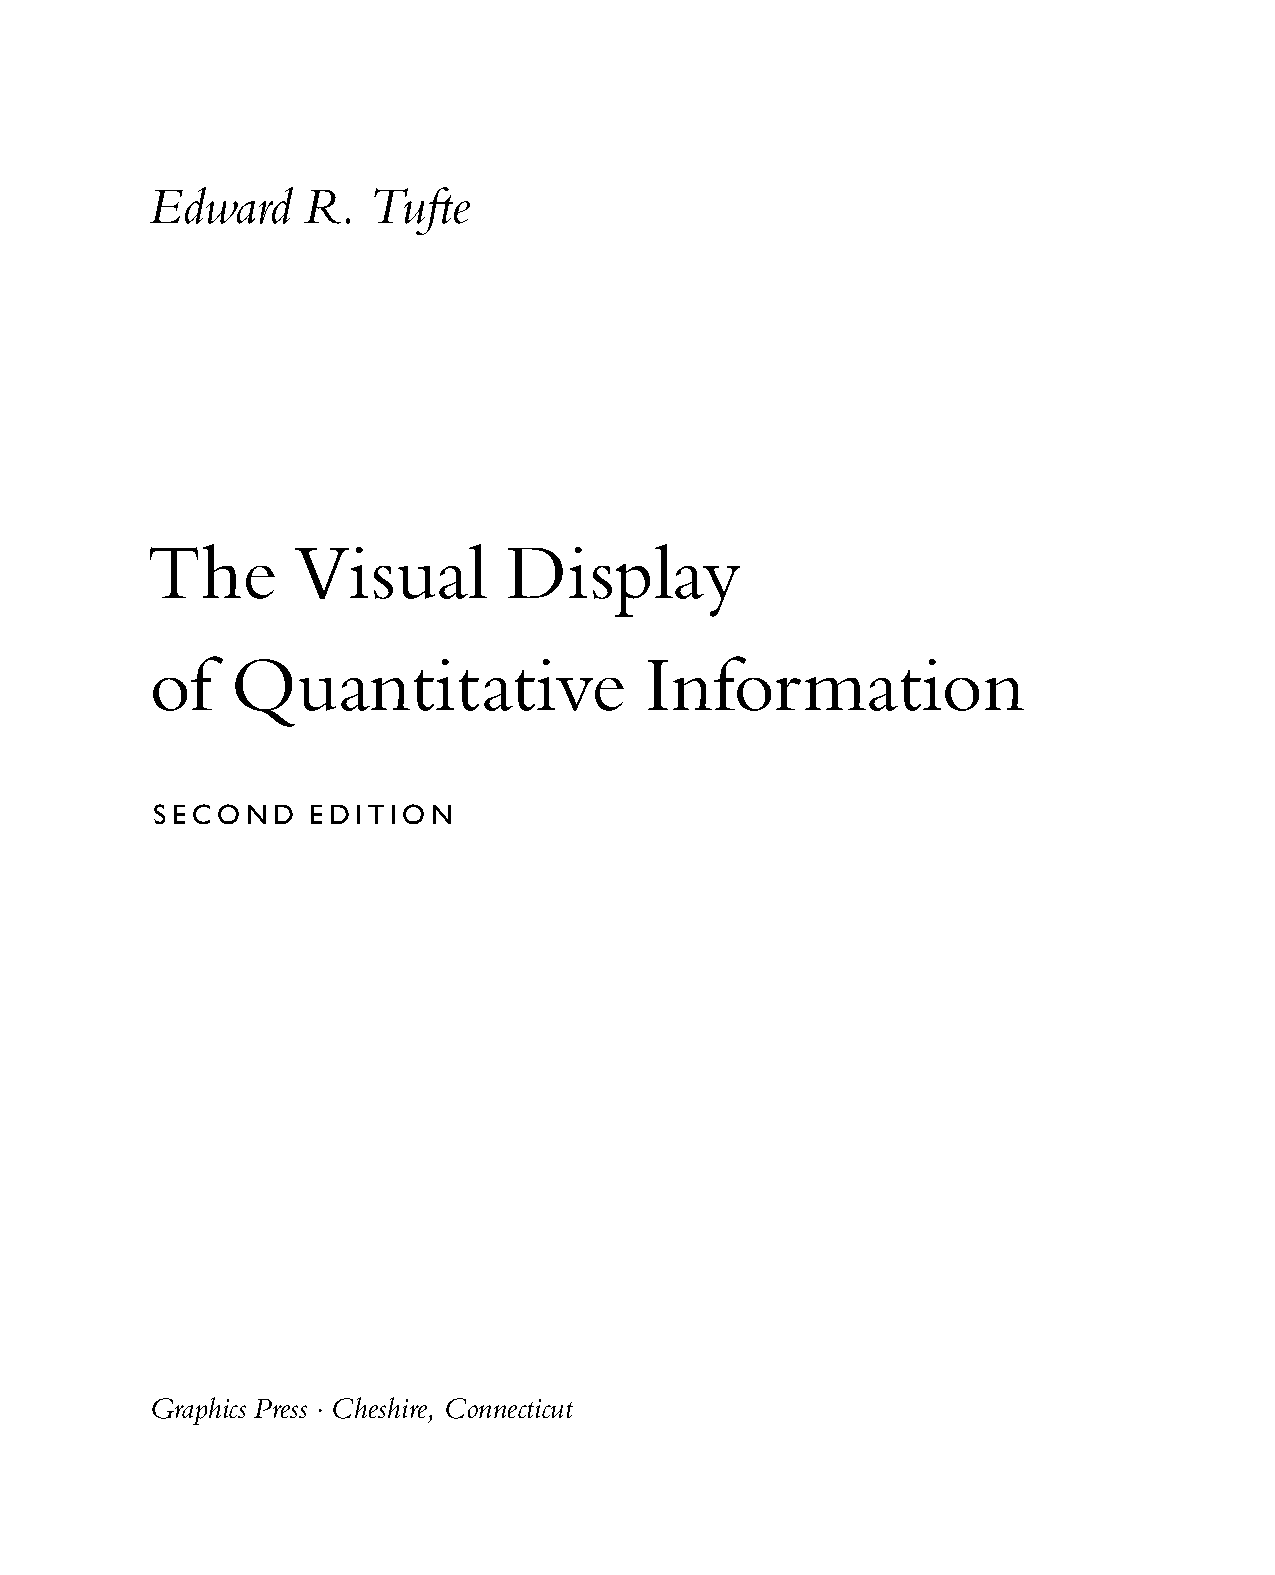
\includegraphics[width=0.45\linewidth]{graphics/vdqi-title.pdf}}
\hfill
\fbox{
\includegraphics[width=0.45\linewidth]{graphics/ei-title.pdf}}
\\\vspace{\baselineskip}
\fbox{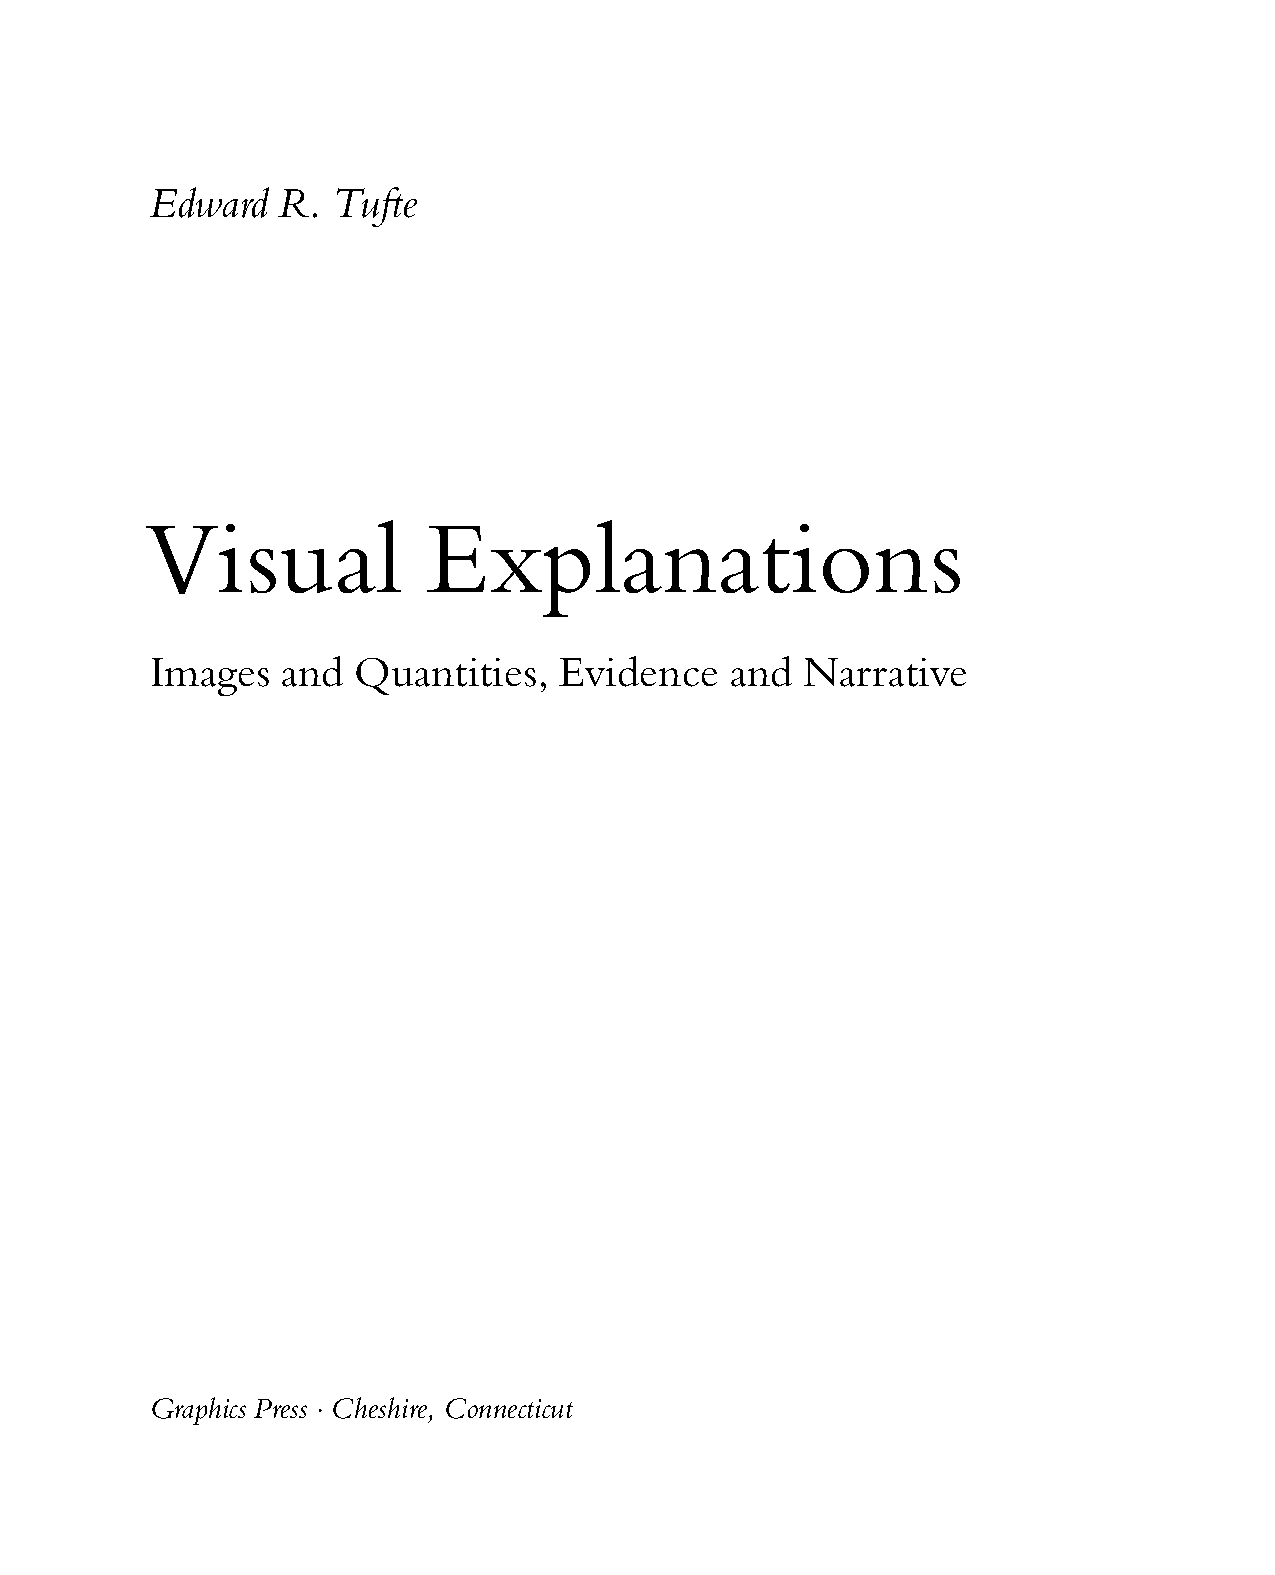
\includegraphics[width=0.45\linewidth]{graphics/ve-title.pdf}}
\hfill
\fbox{
\includegraphics[width=0.45\linewidth]{graphics/be-title.pdf}}
\end{figure*}

\begin{figure*}[p]\index{table of contents}
\fbox{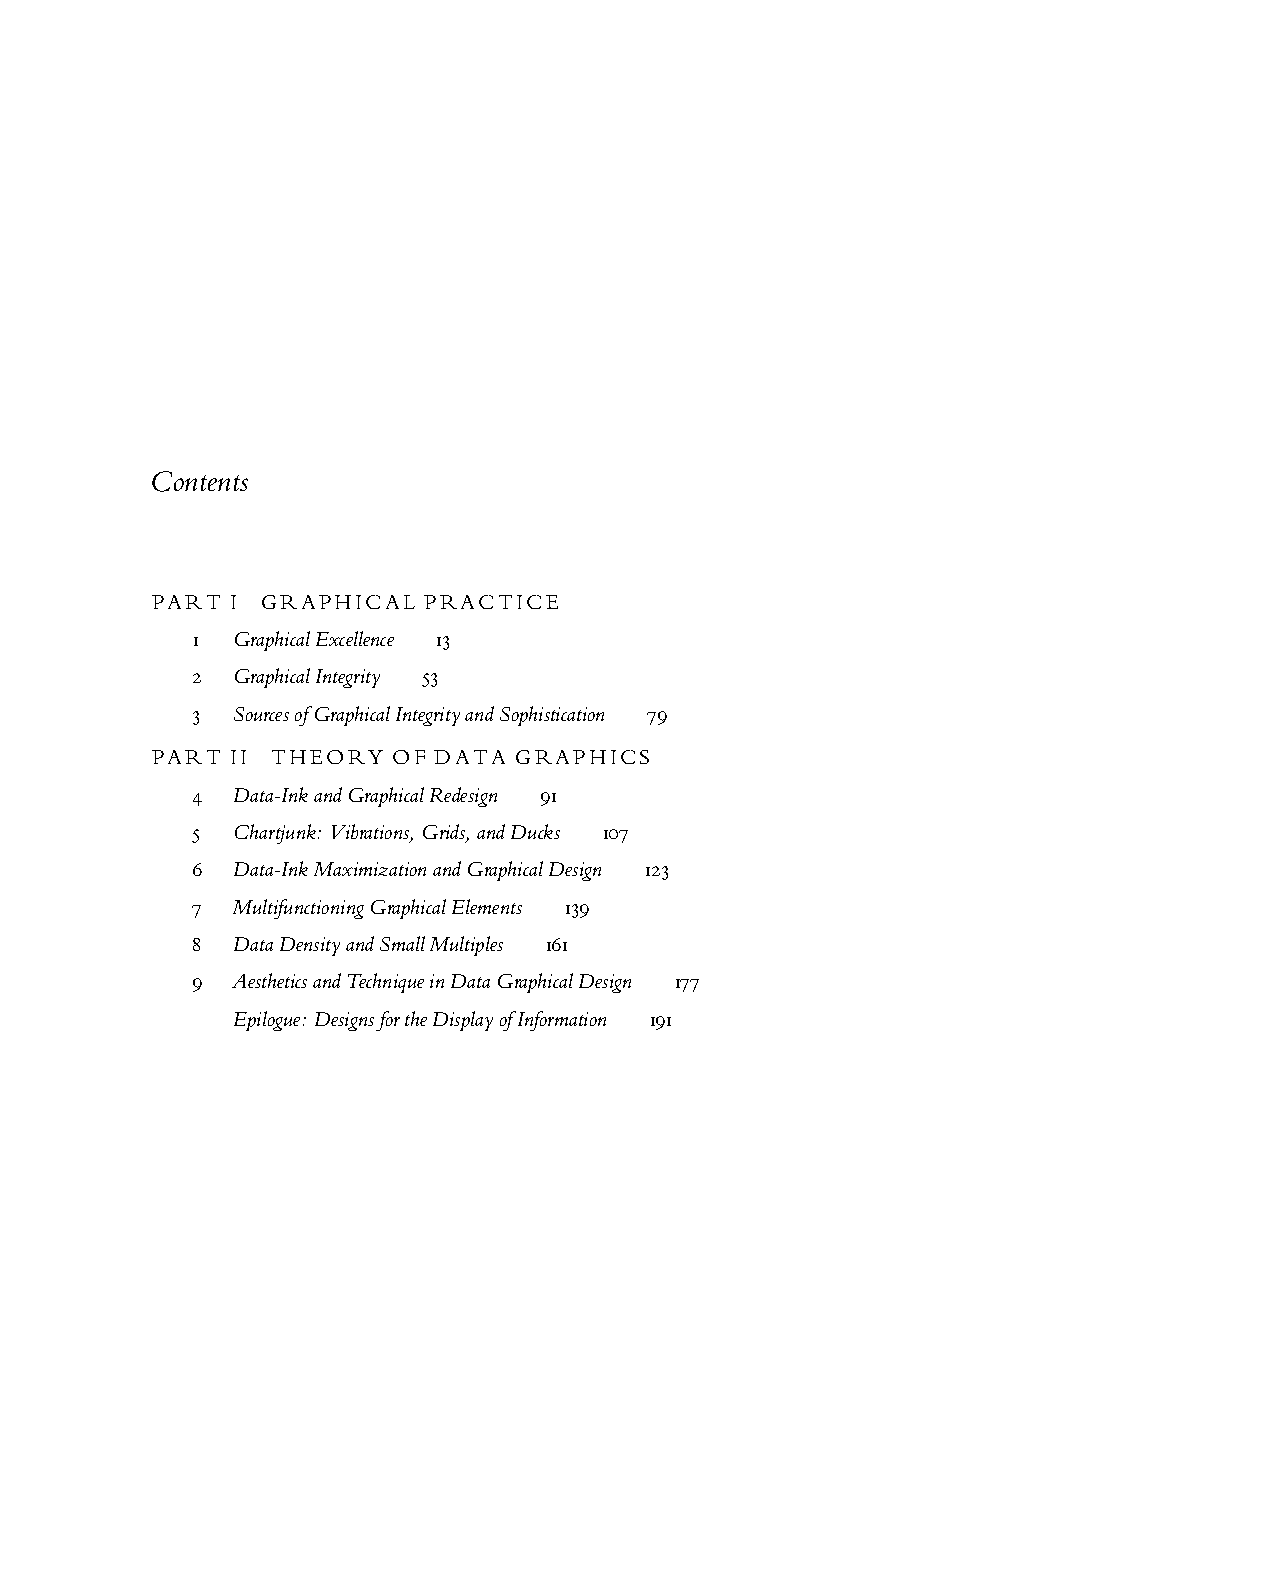
\includegraphics[width=0.45\linewidth]{graphics/vdqi-contents.pdf}}
\hfill
\fbox{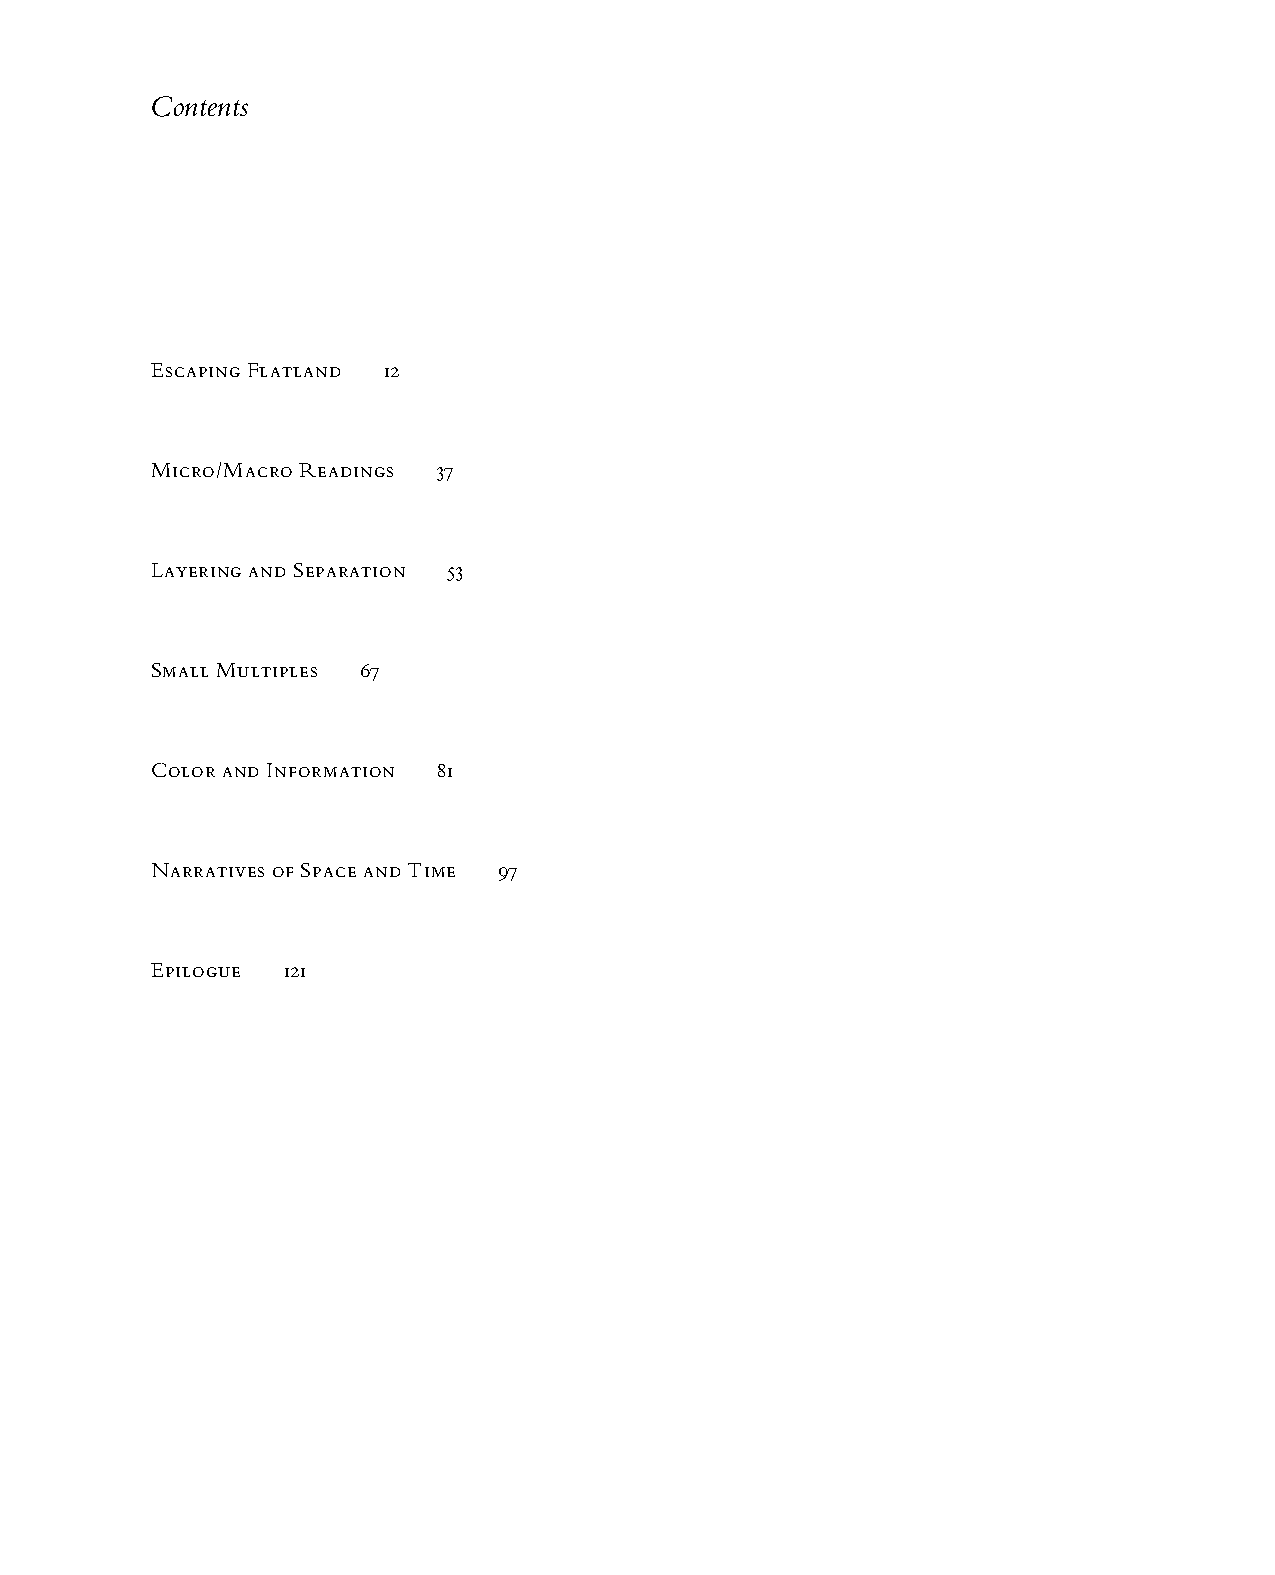
\includegraphics[width=0.45\linewidth]{graphics/ei-contents.pdf}}
\\\vspace{\baselineskip}
\fbox{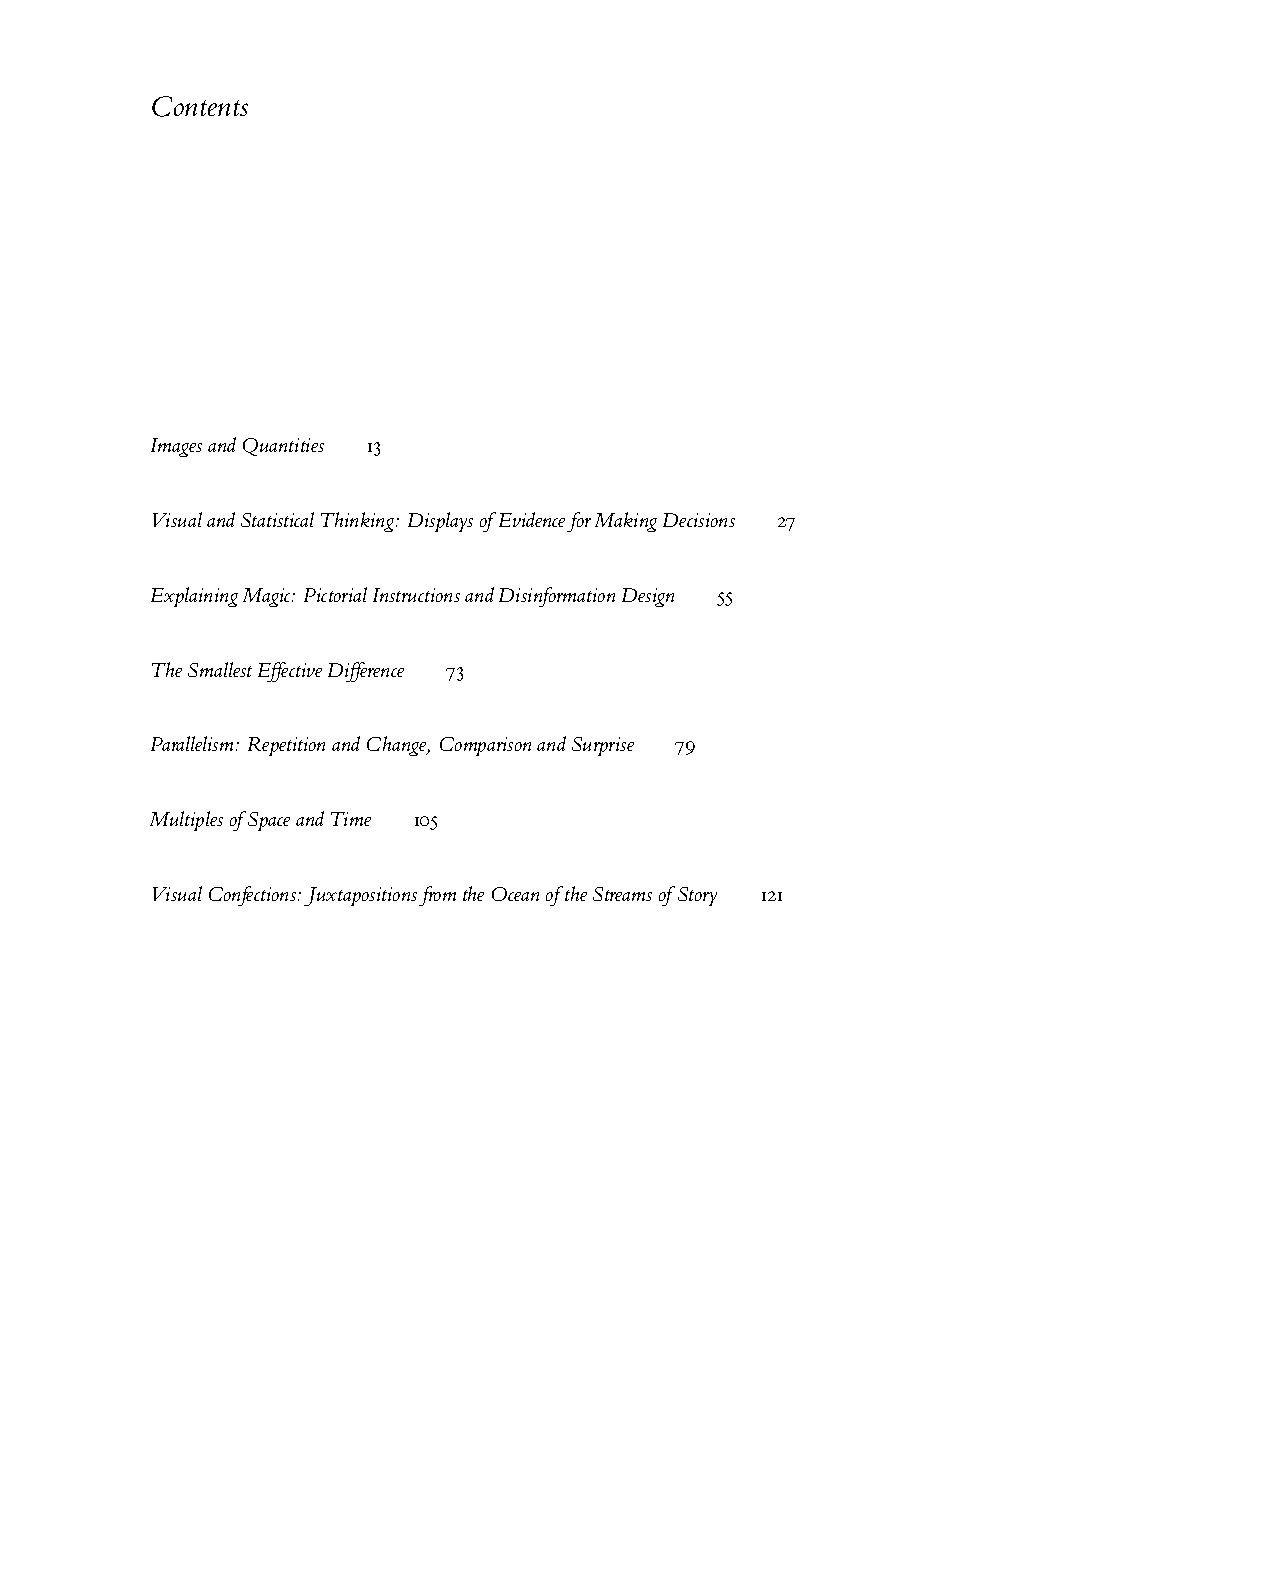
\includegraphics[width=0.45\linewidth]{graphics/ve-contents.pdf}}
\hfill
\fbox{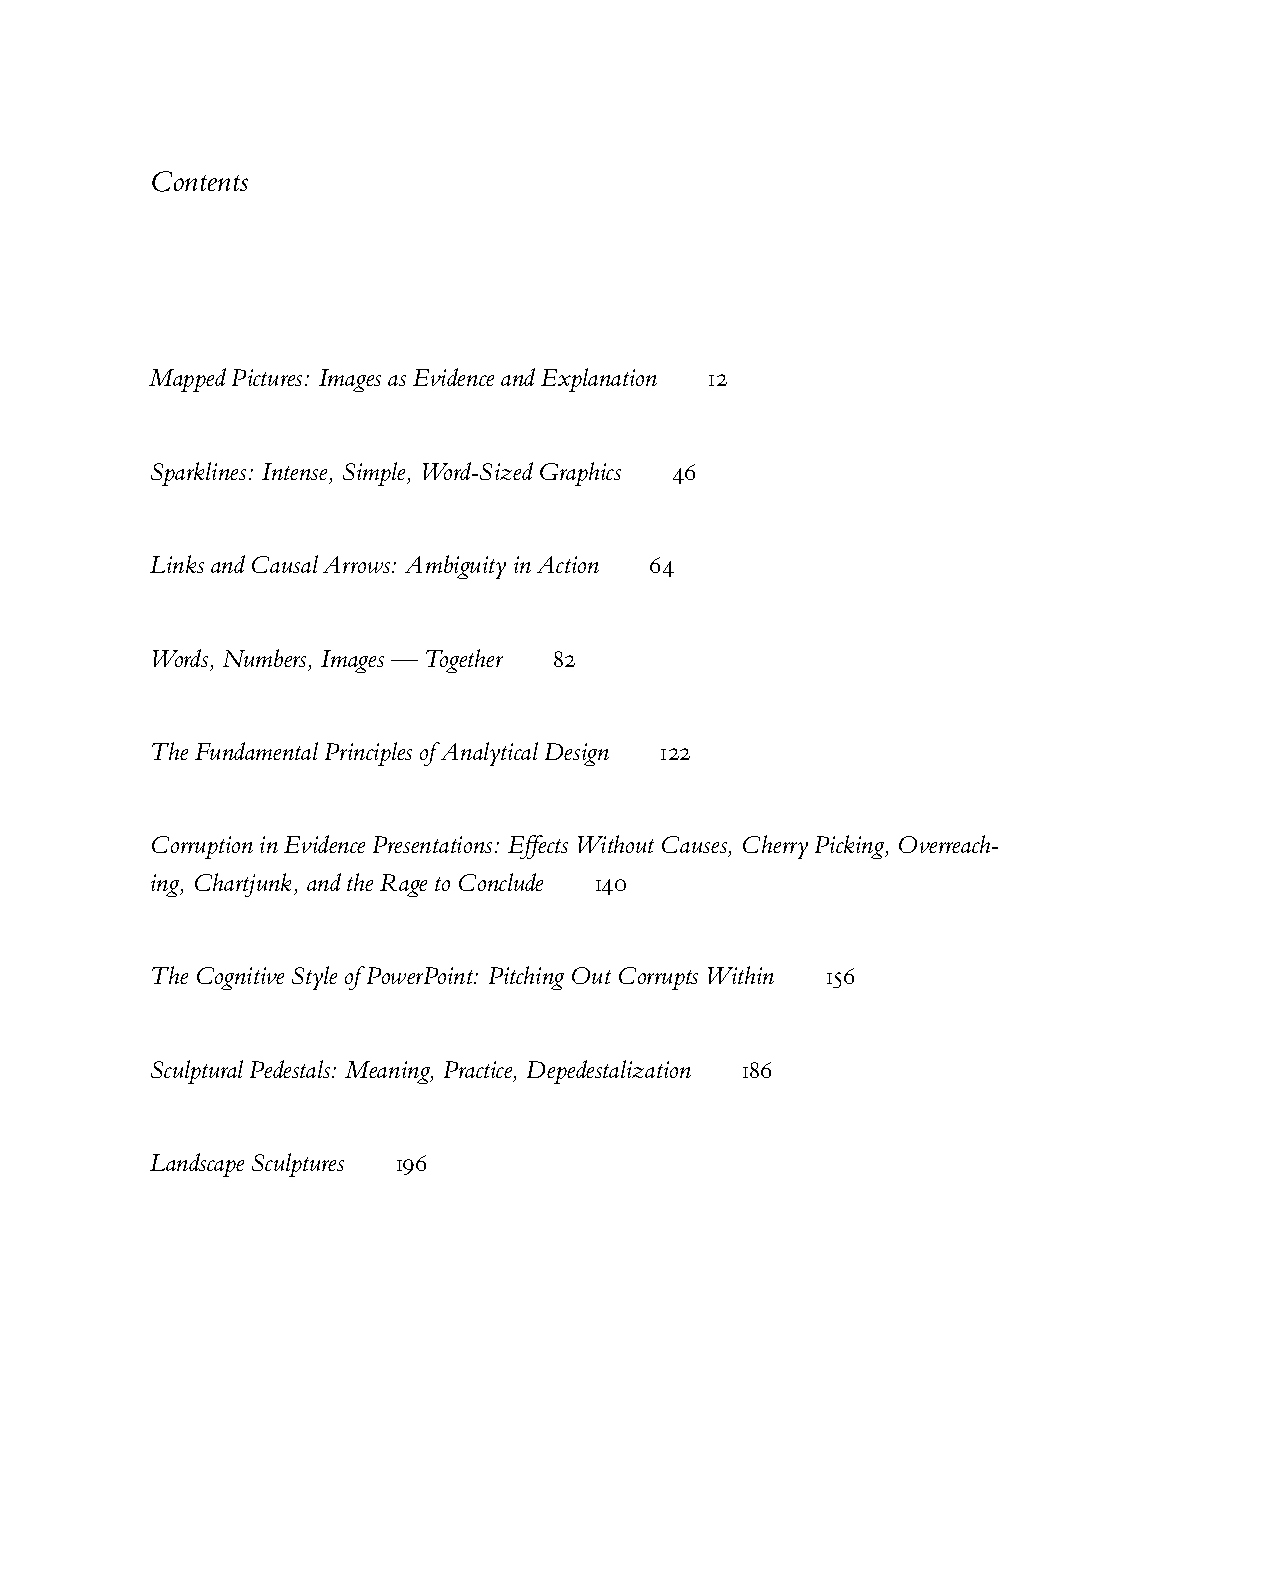
\includegraphics[width=0.45\linewidth]{graphics/be-contents.pdf}}
\end{figure*}


% Index typefaces and fonts, refer from fonts to typefaces
\section{Typefaces}\label{sec:typefaces}\index{typefaces}\index{fonts|see{typefaces}}
\newthought{Tufte's books primarily use two typefaces:} Bembo and Gill Sans.
Bembo is used for the headings and body text, while Gill Sans is used for the title page and opening epigraphs in \BE.

Older versions of \TL\ used Palatino, Helvetica, and Bera Mono fonts.
This version of \TL\ uses \docpkgdef{ETbb} for a Bembo-like font, \docpkgdef{mathpazo} for Palatino math font, \docpkgdef{gillius} for a \textsf{Gill Sans-like font}, and \docpkgdef{FiraMono} as a \texttt{monospaced font}.

However this sample book overrides the default \docpkg{FiraMono} it with \texttt{RecursiveMono} font.
It uses the provided \docfilehook{custom-tufte-common.tex}{common} file hook to override the default font.
I have done that because I like the Recursive Mono font better.
Sadly Recursive font is not available on CTAN, therefore I have used FiraMono as a default font.
If you wish to use Recursive font, you can use font files provided in this package in the \texttt{fonts} directory.

While \TL\ class tries to make documents compiled with \iXeLaTeX, \iLuaLaTeX, and \iPdfLaTeX\ look as similar as possible, it's impossible to make them look identical.
There seem to be small differences between how the engines typeset text, encode fonts, and while \hologo{pdfLaTeX} uses \docpkgdef{fontspec}, the other use \docpkgdef{fontenc}.

\begin{table}[h]\index{typefaces!sizes}
  \footnotesize%
  \begin{center}
    \begin{tabular}{lccl}
      \toprule
      \hologo{LaTeX} size & Font size & Leading & Used for \\
      \midrule
      \Verb|\tiny|         &  5       &  6      & sidenote numbers \\
      \Verb|\scriptsize|   &  7       &  8      & \na{} \\
      \Verb|\footnotesize| &  8       & 10      & sidenotes, captions \\
      \Verb|\small|        &  9       & 12      & quote, quotation, and verse environments \\
      \Verb|\normalsize|   & 10       & 14      & body text \\
      \Verb|\large|        & 11       & 15      & \textsc{b}-heads \\
      \Verb|\Large|        & 12       & 16      & \textsc{a}-heads, \textsc{toc} entries, author, date \\
      \Verb|\LARGE|        & 14       & 18      & handout title \\
      \Verb|\huge|         & 20       & 30      & chapter heads \\
      \Verb|\Huge|         & 24       & 36      & part titles \\
      \bottomrule
    \end{tabular}
  \end{center}
  \caption{A list of \hologo{LaTeX} font sizes as defined by the \TL\ document classes.}\label{tab:font-sizes}
\end{table}


\section{Headings}\label{sec:headings}\index{headings}
\newthought{Tufte's books include the following heading levels:} parts, chapters,%
\sidenote[][-1em]{Parts and chapters are defined for the \texttt{tufte-book} class only.}
sections, subsections, and paragraphs. 
By default subsubsection and subparagraph headings are not defined in the \TL\ classes.
\sidenote[][-0.5em]{For more information on this topic, see~\cite{Bringhurst2005}, section 4.2.2}

\begin{table}[h]
  \begin{center}
    \footnotesize%
    \begin{tabular}{lcr}
      \toprule
      Heading    & Style  & Size \\
      \midrule
      Part       & roman  & \measure{24}{36}{40} \\
      Chapter    & italic & \measure{20}{30}{40} \\
      Section    & italic & \measure{12}{16}{26} \\
      Subsection & italic & \measure{11}{15}{26} \\
      Paragraph  & italic & 10/14 \\
      \bottomrule
    \end{tabular}
  \end{center}
  \caption{Heading styles used in \BE.}\label{tab:heading-styles}
\end{table}

\paragraph{Paragraph} Paragraph headings (as shown here) are introduced by italicized text and separated from the main paragraph by a bit of space.


\section{Environments}
The following table lists characteristics defined for the various environments:

\begin{table}[h]
  \begin{center}
    \footnotesize%
    \begin{tabular}{lcl}
      \toprule
      Environment & Font size            & Notes \\
      \midrule
      Body text   & \measure{10}{14}{26} & \\
      Block quote & \measure{9}{12}{24}  & Block indent (left and right) by \unit[1]{pc} \\
      Sidenotes   & \measure{8}{10}{12}  & Sidenote number is set inline, followed by word space \\
      Captions    & \measure{8}{10}{12}  & \\
      \bottomrule
    \end{tabular}
  \end{center}
  \caption{Environment styles used in \BE.}\label{tab:environment-styles}
\end{table}


% Optional argument changes how the chapter title appears in the TOC
\chapter[On the Use of the tufte-book Document Class]
{On the Use of the \texttt{tufte-book} Document Class}\label{ch:tufte-book}
The \TL\ document classes define a style similar to the style Edward Tufte uses in his books and handouts.
Tufte's style is known for its extensive use of sidenotes, tight integration of graphics with text, and well-set typography.
This document aims to be at once a demonstration of the features of the \TL\ document classes, and a style guide to their use.

\section{Page Layout}\label{sec:page-layout}
\subsection{Headings}\label{ssec:headings}\index{headings}
This style provides \textsc{a}- and \textsc{b}-heads (that is, \doccmddef{section} and \doccmddef{subsection}, demonstrated above).

If you need more than two levels of section headings, you'll have to define them yourself.
This class does not provide pre-defined styles for \doccmddef{subsubsection} or \doccmddef{subparagraph}. 
As Bringhurst points out in \textit{``The Elements of Typographic Style''},\cite{Bringhurst2005} you should ``use as many levels of headings as you need: no more, and no fewer''.

The \TL\ classes will emit an error if you try to use \linebreak\Verb|\subsubsection| or \Verb|\subparagraph|.


\newthought{In his later books},\cite{Tufte2006} Tufte starts each section with a bit of vertical space, a non-indented paragraph, and sets the first few words of the sentence in \textsc{small caps}.
To accomplish this style, use the \doccmddef{newthought} command
\begin{docspec}
  \doccmd{newthought}\{\docarg{In his later books}\}, Tufte starts\ldots
\end{docspec}


\section{Sidenotes}\label{sec:sidenotes}
One of the most prominent and distinctive features of this style is the extensive use of sidenotes.
The wide margin on the right side provides ample room for sidenotes and small figures.
Any \doccmddef{footnote} will automatically be converted into a \doccmd{sidenote}.%
\footnote{This is a sidenote that was entered using the \doccmd{footnote} command.}
If you'd like to place ancillary information in the margin without the sidenote mark (the superscript
number), you can use the \doccmd{marginnote} command.
\marginnote{%
  This is a margin note.
  Notice that there isn't a number preceding the note, and there is no number in the main text where this note was written.
}

In his books Tufte places margin on the right side of the page, regardless whether it's an even or odd page.
If you prefer to alternate the placement of margins, so they fall on outer edge you can use the \docclsopt{symmetric} class option.

\newthought{On a personal note}, placing of sidenotes---be it footnote, citation, or other---should follow the following rules:
\begin{itemize}
  \item If the sidenote applies to the whole sentence, it should be placed after the period or other punctuation mark.
  \item If the sidenote applies to a specific word, it should be placed immediately after that word, even if the word is in the middle of the sentence, or followed by a punctuation mark.
  \item If a sidenote is a complete sentence, or a citation, it should end with a period.
\end{itemize}
The specification of the \doccmddef{sidenote} command is:
\begin{docspec}
  \doccmd{sidenote}[\docopt{number}][\docopt{offset}]\{\docarg{Sidenote text.}\}
\end{docspec}

Both the \docopt{number} and \docopt{offset} arguments are optional.
If you provide a \docopt{number} argument, then that number will be used as the sidenote number.
It will only change the number of the current sidenote, and will not affect the numbering sequence of subsequent sidenotes.

Sometimes a sidenote may run over the top of other text or graphics in the margin space.
If this happens, you can adjust the vertical position of the sidenote by providing a dimension in the \docopt{offset} argument.
Some examples of valid dimensions are:
\begin{docspec}
  \ttfamily 1.0in \qquad 2.54cm \qquad 254mm \qquad 6\Verb|\baselineskip|
\end{docspec}
If the dimension is positive, it will push the sidenote down the page; if the dimension is negative, it will pull the sidenote up the page.

While both the \docopt{number} and \docopt{offset} arguments are optional, they must be provided in order.
To adjust the vertical position of the sidenote while leaving the sidenote number alone, use the following syntax:
\begin{docspec}
  \doccmd{sidenote}[][\docopt{offset}]\{\docarg{Sidenote text.}\}
\end{docspec}
The empty brackets tell the \Verb|\sidenote| command to use the default sidenote number.

If you \emph{only} want to change the sidenote number, however, you may completely omit the \docopt{offset} argument:
\begin{docspec}
  \doccmd{sidenote}[\docopt{number}]\{\docarg{Sidenote text.}\}
\end{docspec}

The \doccmddef{marginnote} command has a similar \docarg{offset} argument:
\begin{docspec}
  \doccmd{marginnote}[\docopt{offset}]\{\docarg{Margin note text.}\}
\end{docspec}

\section{References}
References are placed alongside their citations as sidenotes, as well.
This can be accomplished using the normal \doccmddef{cite} command or the \doccmddef{autocite} command, which functions similarly.%
\sidenote{%
  If you use the \doccmd{cite} command within a sidenote, it will render as an in-line parenthetical citation, as demonstrated here \autocite{Tufte2001}.
}

You will need to specify a bibliography resource file in the preamble of your document using \doccmddef{addbibresource}\{\docarg{bibliography-file.bib}\} command.
The complete list of references may be printed automatically by using the \doccmddef{printbibliography} command.
See the end of this document for an example, and the \iBibLaTeX\ documentation for more information.
Bibliography can be turned off with the help of \docclsopt{nobib} class option.

To enter multiple citations at one location,\autocite{Tufte2006,Tufte1990} you can provide a list of keys separated by commas: 
\begin{docspec}
  \doccmd{cite}\{\docarg{bibkey1,bibkey2,\ldots}\}
\end{docspec}

\newthought{In the new version of \TL}, it's impossible to offset citation's position the same way sidenotes can be moved up or down the margin.
This is caused by the change from \docpkgdef{natbib} package and \hologo{BibTeX} tool to \docpkgdef{biblatex} package and \hologo{biber} tool.
The \docpkg{biblatex} provides it own optional arguments for the \doccmd{cite} commands, which are kept unchanged to avoid confusion.
I see the possible breakage of old \TL\ documents as a fair tradeoff for the new features and flexibility that \docpkg{biblatex} provides.
It is worth noting that the \docpkg{natbib} is mostly kept on life support, so it's better to switch now and make \TL\ more maintainable in the future.
This is one of the reasons why this version of \TL\ classes has a new major version number.


\section{Figures and Tables}\label{sec:figures-and-tables}
Images and graphics play an integral role in Tufte's work.
In addition to the standard \docenvdef{figure} and \docenvdef{tabular} environments, this style provides special figure and table environments for full-width floats.

Full page-width figures and tables may be placed in \docenvdef{figure*} or \docenvdef{table*} environments.
To place figures or tables in the margin, use the \docenvdef{marginfigure} or \docenvdef{margintable} environments as follows (see \cref{fig:marginfig}):
\begin{marginfigure}%
  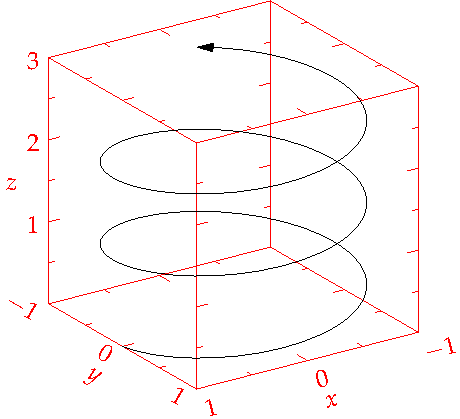
\includegraphics[width=\linewidth]{helix}
  \caption[This is an example of a margin figure]{%
    This is a margin figure. 
    The helix is defined by \(x = \cos(2\pi z)\), \(y = \sin(2\pi z)\), and \(z = [0, 2.7]\). 
    The figure was drawn using \href{http://asymptote.sf.net/}{Asymptote} (\url{http://asymptote.sf.net/}).
  }\label{fig:marginfig}
\end{marginfigure}
\noindent
\begin{Verbatim}
  \begin{marginfigure}
    \includegraphics{margin-figure}
    \caption{Margin figure caption}%
    \label{fig:margin-figure-label}
  \end{marginfigure}
\end{Verbatim}

The \docenv{marginfigure} and \docenv{margintable} environments accept an optional parameter \docopt{offset} that adjusts the vertical position of the figure or table. 
See the ``\nameref{sec:sidenotes}'' section above for examples of how to use offsets.
The specifications are:
\noindent
\begin{Verbatim}[commandchars=+/|]
  \begin{marginfigure}[+docopt/offset|]
    +ldots
  \end{marginfigure}
  +mbox/|
  \begin{margintable}[+docopt/offset|]
    +ldots
  \end{margintable}
\end{Verbatim}

\Cref{fig:fullfig} is an example of the \docenv{figure*} environment and \cref{fig:textfig} is an example of the normal
\docenv{figure} environment.

\begin{figure*}[h]
  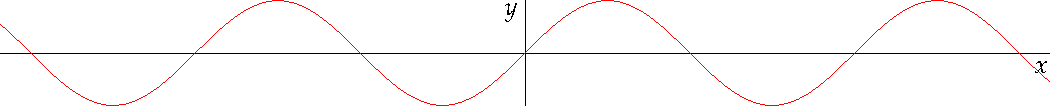
\includegraphics[width=\linewidth]{sine.pdf}%
  \caption[Sine graph showcasing full width figure environment]{%
    This graph shows \(y = \sin x\) from about \(x = [-10, 10]\).
    \emph{Notice that this figure takes up the full page width.}
  }\label{fig:fullfig}
\end{figure*}

\begin{figure}
  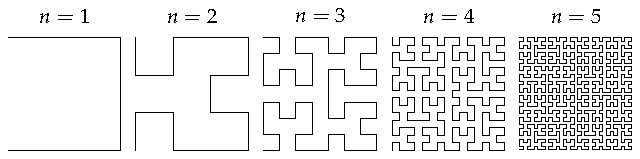
\includegraphics{hilbert-curves.pdf}
  \caption[Hilbert curves of various degrees \(n\)][2em]{%
    Hilbert curves of various degrees \(n\).
    \emph{Notice that this figure only takes up the main textblock width.}
  }\label{fig:textfig}
\end{figure}

\newthought{As with sidenotes and marginnotes}, a caption may require vertical adjustment. 
The \doccmddef{caption} command can take a second optional argument which enables you to do this by providing a dimension \docopt{offset}.
You may specify the caption in any one of the following forms:
\begin{docspec}
  \doccmd{caption}\{\docarg{long caption}\} \\
  \doccmd{caption}[\docarg{short caption}]\{\docarg{long caption}\} \\
  \doccmd{caption}[][\docopt{offset}]\{\docarg{long caption}\} \\
  \doccmd{caption}[\docarg{short caption}][\docopt{offset}]\{\docarg{long caption}\}
\end{docspec}
A positive \docopt{offset} will push the caption down the page.
The short caption, if provided, is what appears in the list of figures/tables, otherwise the ``long'' caption appears there.
Note that although the arguments \docopt{short caption} and \docopt{offset} are both optional, they must be provided in order. 
Thus, to specify an \docopt{offset} without specifying a \docopt{short caption}, you must include the first set of empty brackets \Verb|[]|, which tell \doccmd{caption} to use the default ``long'' caption. 
As an example, the caption to \cref{fig:textfig} above was given in the form:
\begin{docspec}
  \doccmd{caption}[Hilbert curves\ldots][1em]\{Hilbert curves\ldots{}\}
\end{docspec}

\newthought{Note that caption offset is unavailable} for \docenv{marginfigure} and \docenv{margintable} environments.
In these cases you need to offset the whole figure or table.
Captions in \docenv{marginfigure} and \docenv{margintable} still support short captions.

\newthought{Tufte style tables are simple} and should be styled with the \docpkgdef{booktabs} package.
\Cref{tab:normaltab} shows table created with the \docpkg{booktabs} package.
Notice the lack of vertical rules---they serve only to clutter the table's data.
Hence Tufte style tables use only horizontal rules.
In cases where a table has many rows, \docpkgdef{colortbl} can be used to make rows stand out visually from each other.
Colors can be used to group related rows, highlight important data, or make one row stand out from the others.

\begin{table}[ht]
  \centering
  \fontfamily{ppl}\selectfont
  \begin{tabular}{ll}
    \toprule
    Margin & Length \\
    \midrule
    Paper width               & \unit[8\nicefrac{1}{2}]{inches} \\
    Paper height              & \unit[11]{inches} \\
    Textblock width           & \unit[6\nicefrac{1}{2}]{inches} \\
    Textblock/sidenote gutter & \unit[\nicefrac{3}{8}]{inches} \\
    Sidenote width            & \unit[2]{inches} \\
    \bottomrule
  \end{tabular}
  \caption[Dimensions of the margins in \doccls{tufte-handout}]{%
  Here are the dimensions of the various margins used in the Tufte-handout class.%
  }\label{tab:normaltab}
\end{table}


\subsection{Too Many Floats}\label{ssec:too-many-floats}
\newthought{Occasionally} \hologo{LaTeX} will generate an error message:
\begin{docspec}
  Error: Too many unprocessed floats
\end{docspec}
\hologo{LaTeX} tries to place floats in the best position on the page.
Until it's finished composing the page, however, it won't know where those positions are.
If you have a lot of floats on a page (including sidenotes, margin notes, figures, tables, etc.),
\hologo{LaTeX} may run out of ``slots'' to keep track of them and will generate the aforementioned error.

\hologo{LaTeX} initially allocates 18 slots for storing floats. 
To work around this limitation, the \TL\ document classes provide a \doccmddef{morefloats} command that will reserve more slots.

The first time \doccmd{morefloats} is called, it allocates an additional 34 slots.
The second time \doccmd{morefloats} is called, it allocates another 26 slots.

The \doccmd{morefloats} command may only be used two times.
Calling it a third time will generate an error message:
\begin{docspec}
  You may only call \string\morefloats\space twice\\
  See the Tufte-LaTeX documentation for alternatives
\end{docspec}
This is because allocating more floats may lead \hologo{LaTeX} to run out of memory.

If, after using the \doccmd{morefloats} command twice, you continue to get the \texttt{Too many unprocessed floats} error, there are a couple things you can do:

The \doccmddef{FloatBarrier} command will immediately process all the floats before typesetting more material.
Since \doccmd{FloatBarrier} will start a new paragraph, you should place this command at the beginning or end of a
paragraph.

The \doccmddef{clearpage} command will also process the floats before continuing, but instead of starting a new paragraph, it will start a new page.

You can also try moving your floats around a bit: move a figure or table to the next page, or reduce the number of sidenotes.
Keep in mind that each sidenote actually uses \emph{two} float slots.

After placing the floats, \hologo{LaTeX} will mark those slots as unused so they are available for the next page to be composed.


\section{Captions}
You may notice that the captions are sometimes misaligned.
Due to the way \hologo{LaTeX}'s floats works, it's hard to know for sure where it decided to put the float.
Therefore, the \TL\ document classes provide commands to override the caption position.

\paragraph{Vertical alignment}\label{par:vertical-alignment}
In cases where the caption is too high or too low on the page, you can adjust its vertical position.
To override the caption's vertical alignment, use the provided \doccmd{setfloatalignment} command inside the float environment.
For example:

\begin{Verbatim}[commandchars=+/|]
\begin{figure}
  \includegraphics{vertical-figure}
  \caption{vertical-figure-caption}%
  \label{fig:vertical-figure-label}
  +hlorange/\setfloatalignment{b}| % forces caption to be bottom-aligned
\end{figure}
\end{Verbatim}

\noindent The syntax of the \doccmddef{setfloatalignment} command is:

\begin{docspec}
  \doccmd{setfloatalignment}\{\docopt{pos}\}
\end{docspec}

\noindent where \docopt{pos} can be either \texttt{b} for bottom-aligned captions, or \texttt{t} for top-aligned captions.

\paragraph{Horizontal alignment}\label{par:horizontal-alignment}
To override the horizontal alignment, use either the \doccmd{forceversofloat} or the \doccmd{forcerectofloat} command inside of the float environment.
Note that these commands only work when the \docclsopt{symmetric} option is enabled.
For example:

\begin{Verbatim}[commandchars=+/|]
\begin{figure}
  \includegraphics{horizontal-figure}
  \caption{horizontal-figure-caption}%
  \label{fig:horizontal-figure-label}
  +hlorange/\forceversofloat| % forces caption to the left of the float
\end{figure}
\end{Verbatim}

\noindent The \doccmddef{forceversofloat} command causes the algorithm to assume the float has been placed on a verso page---that is, a page on the left side of a two-page spread.
Conversely, the \doccmddef{forcerectofloat} command causes the algorithm to assume the float has been placed on a recto page---that is, a page on the right side of a two-page spread.


\section{Full-width text blocks}
In addition to the new float types, there is a \docenvdef{fullwidth} environment.
This environment stretches across the main text block and the sidenotes area.

\begin{Verbatim}[commandchars=+/|]
\begin{fullwidth}
  Lorem ipsum dolor sit amet+ldots
\end{fullwidth}
\end{Verbatim}

\begin{fullwidth}
\small\itshape\lipsum[1]
\end{fullwidth}


\section{Typography}\label{sec:typography}
\subsection{Typefaces}\label{ssec:typefaces}%
% Index typefaces and fonts, refer from fonts to typefaces
\index{typefaces}\index{fonts|see{typefaces}}

When using \iXeLaTeX\ or \iLuaLaTeX, the \TL\ classes will load the \docpkg{fontspec} package.
This package allows you to set the typeface to any installed font, any local font files, or to any font files you have installed in your \texttt{TEXMF} tree.

By default the \TL\ classes will use the ET-Bembo font from the \docpkg{ETbb} package, as the main typeface.
If it's unavailable, the \TeX\ Gyre Pagella from the \docpkg{tex-gyre-pagella} package will be used as fallback serif font.
For math fonts it tries to use the Palatino font from the \docpkg{mathpazo} package.
For sans serif text the \textsf{Gillius No. 2} font from the \docpkg{gillius} package will be used.
If this one is unavailable, the \TeX\ Gyre Heros font from the \docpkg{tex-gyre-heros} package will be used.
In case of monospaced text the \texttt{Fira Mono} font from the \docpkg{FiraMono} package will be used.
If it's not present, the \TeX\ Gyre Cursor font from the \docpkg{tex-gyre-cursor} package will be used.
However the provided \docfilehook{custom-tufte-common.tex}{common} file hook overrides the default monospaced font with \texttt{RecursiveMono} font.
This file shows how you can override the default fonts, and how the file hooks can be used.

The \TeX\ Gyre faces are usually included with \TeX\ Live distributions, hence why they are used as fallback fonts.
If any of the selected fonts don't suit you, you can easily change them using the \docpkg{fontspec} package.

\newthought{When using the} \iPdfLaTeX\ engine, the \TL\ classes will try to use the same default fonts, but will fall back to the default Computer Modern fonts if they are unavailable.
The \docpkg{fontspec} package is not available under \hologo{pdfLaTeX}, so it uses the \docpkg{fontenc} package to set the font encoding.
This package doesn't make it easy to use non-standard fonts, so it's recommended to use \iXeLaTeX\ or \iLuaLaTeX\ for the best results.
Alternatively install and use font packages that are compatible with \hologo{pdfLaTeX}.

\newthought{In cases where} \docclsopt{nofonts} option is used, the \TL\ classes will not load any fonts.
It will not load \docpkg{fontspec} or \docpkg{fontenc} packages either.%
In \hologo{LuaLaTeX} or \hologo{XeLaTeX} both \docclsopt{nofonts} \textbf{and} \docclsopt{nols} must be used to disable loading \docpkg{fontspec}. More info in \nameref{ssec:letterspacing} section.

\subsection{Letterspacing}\label{ssec:letterspacing}
This document class includes two new commands and some improvements on existing commands for letterspacing.

When setting strings of \allcaps{ALL CAPS} or \smallcaps{small caps} commands, the letter\-spacing---that is, the spacing between the letters---should be increased slightly.\cite{Bringhurst2005}
The \doccmddef{allcaps} command was modified with proper letterspacing for strings of \allcaps{full capital letters}, and the \doccmddef{smallcaps} command was modified with spacing for \smallcaps{SMALL CAPITAL LETTERS}.
These commands will also automatically convert the case of the text to upper- or lowercase, respectively.
You can see that in the source code of this document.

The \doccmddef{textsc} command has also been redefined to include proper letterspacing.
However, the case of the \doccmd{textsc} argument is left as is.
This allows one to use both uppercase and lowercase letters:
\textsc{The Initial Letters Of The Words In This Sentence Are Capitalized.}


%%% TODO: Continue from here
\section{Document Class Options}\label{sec:options}%
% Second index command opens the class options index span
\index{options|see{class options}}\index{class options|(}
The \doccls{tufte-book} class is based on the \hologo{LaTeX} \doccls{book} document class.
Conversely the \doccls{tufte-handout} class is based on the \doccls{article} document class.
Therefore, you can pass any of the typical book or article options to them.
There are a few options that are specific to the \doccls{tufte-book} and \doccls{tufte-handout} document classes, however.

\subsection{Paper Size and Layout Options}\label{ssec:paper-size-layout-options}
The \docclsoptdef{a4paper} option will set the paper size to \smallcaps{A4} instead of the default \smallcaps{US} letter size.

The \docclsoptdef{b5paper} option will set the paper size to \smallcaps{B5} instead of the default \smallcaps{US} letter size.

The \docclsopt{a5paper}, \docclsopt{executivepaper}, and \docclsopt{legalpaper} options are unavailable in the \TL\ classes.

The \docclsoptdef{twoside} option will modify the running heads so that the page number is printed on the outside edge. By default \TL\ classes always print the page number on the right-side edge.

The \docclsoptdef{symmetric} option typesets the sidenotes on the outside edge of the page.
This is how books are traditionally printed, but is contrary to Tufte's book design which sets the sidenotes on the right side of the page.
This option implicitly sets the \docclsopt{twoside} option.

The \docclsopt{landscape}, \docclsopt{onecolumn}, and \docclsopt{twocolumn} options are not available in the \TL\ classes.

\subsection{Font and Text Options}\label{ssec:font-options}
The \docclsoptdef{sftitle} option will set the title page and title block in a \textsf{sans serif} typeface.
The \docclsoptdef{nosftitle} option will set the title page and title block in a serif typeface.
In case of \doccls{tufte-handout} these options also have an effect on the abstract.
While in \doccls{tufte-book} they affect the epigraphs.
By default the \doccls{tufte-book} class uses \docclsopt{sftitle} and the \doccls{tufte-handout} class uses \docclsopt{nosftitle}.

The \docclsoptdef{sfmarginals} option makes all marginals use \textsf{sans serif} typeface instead of the default roman typeface.

The \docclsoptdef{justified} option sets all the text fully justified (flush left and right). 
The default is to set the text ragged right.
The body text of Tufte's books are set ragged right. 
This prevents needless hyphenation and makes it easier to read the text in the slightly narrower column.

The \docclsopt{10pt}, \docclsopt{11pt}, and \docclsopt{12pt} options are unavailable in the \TL\ classes.

The \docclsoptdef{nofonts} option prevents the \TL\ classes from automatically loading the Tufte typefaces
You should use this option if you wish to load your own fonts in \iPdfLaTeX. 
If you're using \iXeLaTeX\ or \iLuaLaTeX, the will not be loaded, and you can use \docpkg{fontspec} to set your own.
If you aren't using the \docclsopt{nols} option, the \docpkg{fontspec} package will be loaded as it is required for letterspacing. 

The \docclsoptdef{nols} option inhibits the letterspacing code. 
The \TL\ classes try to load the appropriate letterspacing package to adjust spacing of letters.
It uses \docpkg{letterspace} or the \docpkg{soul} under \hologo{pdfLaTeX}.
In case of \hologo{XeLaTeX} and \hologo{LuaLaTeX} it uses \docpkg{fontspec}.

The \docclsoptdef{bidi} option loads the \docpkg{bidi} package which is used with \hologo{XeLaTeX} to typeset bi-directional text. 
Since the \docpkg{bidi} package needs to be loaded before the sidenotes and cite commands are defined, it can't be loaded in the document preamble.

\subsection{Title Page Options}\label{ssec:title-page-options}
The \docclsoptdef{notitlepage} option causes \doccmd{maketitle} to generate a title block instead of a title page. 
By default the \doccls{tufte-book} class uses \docclsopt{titlepage} and the \doccls{tufte-handout} class uses \docclsopt{notitlepage}.
There is an analogous \docclsoptdef{titlepage} option that forces \doccmd{maketitle} to generate a full title page instead of the title block.

\subsection{Toggle Options}\label{ssec:toggle-options}
The \docclsoptdef{nobib} option inhibits loading of the \docpkg{natbib} and \docpkg{bibtex} packages and modification of the \doccmd{cite} command.

The \docclsoptdef{notoc} option suppresses \TL's custom table of contents (\textsc{toc}) design.
The current \textsc{toc} design only shows unnumbered chapter titles in books; it doesn't show sections or subsections. 
The \docclsopt{notoc} option will revert to \hologo{LaTeX}'s \textsc{toc} design.

The \docclsoptdef{nohyper} option prevents the \docpkg{hyperref} package from being loaded.
The default is to load the \docpkg{hyperref} package and use the \doccmd{title} and \doccmd{author} contents as metadata for the generated \textsc{pdf}.

The \docclsoptdef{nomoderntitles} is a new option added in the latest version of \TL.
It only works in the \doccls{tufte-handout} class.
It disables coloring and styling of the section and paragraph titles.
The default is to color the titles and add a colored box to the left with section numbers.

\subsection{Marginal Options}\label{ssec:marginal-options}
In the \TL\ classes there are four types of marginal materials, which are:
\docclsoptdef{sidenote}, \docclsoptdef{marginnote}, \docclsoptdef{caption}, and \docclsoptdef{citation}.
Each of those can have their justification set to one of the following options:
\begin{description}
  \item[\docclsopt{justified}] Fully justifies the text (sets it flush left and right).
  \item[\docclsopt{raggedleft}] Sets the text ragged left.
  \item[\docclsopt{raggedright}] Sets the text ragged right.
  \item[\docclsopt{raggedouter}] Sets the text ragged left if on the left-hand (verso) page, otherwise ragged right.
  This is useful in conjunction with the \docclsopt{symmetric} document class option.
  \item[\docclsopt{auto}] Fully justifies the text if \docclsopt{justified} class option was specified, otherwise the text is set ragged right.
  This is the default justification option for marginal material.
\end{description}

Additionally, the \docclsoptdef{marginals} option can be used to set the justification settings for all marginal texts.
See the \nameref{sec:customizing-marginal-material} section for more information on marginal material.

\subsection{Debugging Options}\label{ssec:debugging-options}
The \docclsoptdef{debug} option causes the \TL\ classes to output debug information to the log file which is useful in troubleshooting bugs.
It prints list of options and their values under the \texttt{Tufte-LaTeX settings} section.
It will also cause the graphics to be replaced by outlines.
When combined with \doccmd[geometry]{geometry}\docopt{showframe} command it will show margins for debugging page layout issues.%
% This command ends the class options index span which started at the beginning of the section
\index{class options|)}


\chapter[Customizing Tufte-LaTeX]{Customizing \TL}\label{ch:customizing}
The \TL\ document classes are designed to closely emulate Tufte's book design by default.
However, each document is different and you may encounter situations where the default settings are insufficient.
This chapter explores many of the ways you can adjust the \TL\ document classes to better fit your needs.

\section{File Hooks}\label{sec:filehooks}%
\index{file hooks|(}
When creating many documents using the \TL\ classes, it's easier to store customizations in one file.
Otherwise they would need to be copied into the preamble of each document.
The \TL\ classes provide three file hooks: \docfilehook{custom-tufte-common.tex}{common}, \docfilehook{custom-tufte-book.tex}{book}, and \docfilehook{custom-tufte-handout.tex}{handout}.\sloppy

\begin{description}
  \item[\docfilehook{custom-tufte-common.tex}{common}]
    If this file exists, it will be loaded by all of the \TL\ document classes, just prior to any class-specific code. If your customizations or code should be included in both the book and handout classes, use this file hook.
  \item[\docfilehook{custom-tufte-book.tex}{book}] 
    If this file exists, it will be loaded after all of the common and book-specific code has been read. 
    If your customizations apply only to the book class, use this file hook.
  \item[\docfilehook{custom-tufte-handout.tex}{handout}] 
    If this file exists, it will be loaded after all of the common and handout-specific code has been read.
    If your customizations apply only to the handout class, use this file hook.
\end{description}%
\index{file hooks|)}


\section{Numbered Section Headings}\label{sec:numbered-sections}%
\index{headings!numbered}
While Tufte dispenses with numbered headings in his books, if you require them, they can be enabled by changing the value of the \doccounter{secnumdepth}counter. 
From the table below, select the heading level at which numbering should stop and set the \doccounter{secnumdepth} counter to that value.
For example, if you want parts and chapters numbered, but don't want numbering for sections or subsections, use the command:
\begin{docspec}
  \doccmd{setcounter}\{secnumdepth\}\{0\}
\end{docspec}

The default value of \doccounter{secnumdepth} for the \doccls{tufte-book} class is \(-1\).
This version of \doccls{tufte-handout} class sets the counter to \(2\) so sections and subsections are numbered.
This change was made to make the sections stand out more as I found it hard to distinguish them from the body text.
If you wish to revert to no numbering, set the counter to \(-1\).
You can also pass the \docclsopt{nomoderntitles} option to the \doccls{tufte-handout} class to disable the coloring and styling of the section and paragraph titles.

\begin{table}
  \footnotesize
  \begin{center}
    \begin{tabular}{lr}
      \toprule
      Heading level                         & Value \\
      \midrule
      Part (in \doccls{tufte-book})         & \(-1\) \\
      Part (in \doccls{tufte-handout})      & \(0\) \\
      Chapter (only in \doccls{tufte-book}) & \(0\) \\
      Section                               & \(1\) \\
      Subsection                            & \(2\) \\
      Subsubsection                         & \(3\) \\
      Paragraph                             & \(4\) \\
      Subparagraph                          & \(5\) \\
      \bottomrule
    \end{tabular}
  \end{center}
  \caption{Heading levels used with the \texttt{secnumdepth} counter.}
\end{table}


\section{Changing the Paper Size}%
\label{sec:paper-size}

The \TL\ classes currently only provide three paper sizes: \textsc{A4}, \textsc{B5}, and \textsc{US} letter.
To specify a different paper size (and/or margins), use the \doccmd[geometry]{geometry} command in the preamble of your
document (or one of the file hooks).
The full documentation of the \doccmd{geometry} command may be found in the \docpkg{geometry} package documentation.%
\cite{pkg-geometry}


\section{Customizing Marginal Material}\label{sec:customizing-marginal-material}
Marginal material includes sidenotes, citations, margin notes, and captions.
Normally, the justification of the marginal material follows the justification of the body text. 
If you specify the \docclsopt{justified} document class option, all of the margin material will be fully justified as well. 
If you don't specify the \docclsopt{justified} option, then the marginal material will be set ragged right.

You can set the justification of the marginal material separately from the body text using the following document class options: \docclsopt{sidenote}, \docclsopt{marginnote}, \docclsopt{caption}, \docclsopt{citation}, and \docclsopt{marginals}. 
Each option refers to its obviously corresponding marginal material type. 
The \docclsopt{marginals} option simultaneously sets the justification on all four marginal material types.

Each of the document class options takes one of five justification types:
\begin{description}
  \item[\docclsopt{justified}] Fully justifies the text (sets it flush left and right).
  \item[\docclsopt{raggedleft}] Sets the text ragged left, regardless of which page it falls on.
  \item[\docclsopt{raggedright}] Sets the text ragged right, regardless of which page it falls on.
  \item[\docclsopt{raggedouter}] Sets the text ragged left if it falls on the left-hand (verso) page of the spread and otherwise sets it ragged right.
  This is useful in conjunction with the \docclsopt{symmetric} document class option.
  \item[\docclsopt{auto}] If the \docclsopt{justified} document class option was specified, then set the text fully justified; otherwise the text is set ragged right. 
  This is the default justification option if one is not explicitly specified.
\end{description}

\noindent For example, 
\begin{docspec}
  \doccmdnoindex{documentclass}[symmetric,justified,marginals=raggedouter]\{tufte-book\}
\end{docspec}
will set the body text of the document to be fully justified.
All of the margin material (sidenotes, margin notes, captions, and citations) to be flush against the body text with ragged outer edges.

\newthought{The font and style} of the marginal material may also be modified using the following commands:

\begin{docspec}
  \doccmd{setsidenotefont}\{\docopt{font commands}\} \\
  \doccmd{setcaptionfont}\{\docopt{font commands}\} \\
  \doccmd{setmarginnotefont}\{\docopt{font commands}\} \\
  \doccmd{setcitationfont}\{\docopt{font commands}\}
\end{docspec}

The \doccmddef{setsidenotefont} sets the font and style for sidenotes, the \doccmddef{setcaptionfont} for captions, the \doccmddef{setmarginnotefont} for margin notes, and the \doccmddef{setcitationfont} for citations. 
The \docopt{font commands} can contain font size changes (e.g., \doccmdnoindex{footnotesize}, \doccmdnoindex{Huge}, etc.), font style changes (e.g., \doccmdnoindex{sffamily}, \doccmdnoindex{ttfamily}, \doccmdnoindex{itshape}, etc.), color changes (e.g., \doccmdnoindex{color}\texttt{\{tufte-blue\}}), and many other adjustments.

If, for example, you wanted the captions to be set in italic sans serif, you could use:
\begin{docspec}
  \doccmd{setcaptionfont}\{\doccmdnoindex{itshape}\doccmdnoindex{sffamily}\}
\end{docspec}


\chapter{Compatibility Issues}\label{ch:compatibility}
When switching an existing document from one document class to a \TL\ document class, a few changes to the document may have to be made.


\section{Converting from \doccls{article} to \doccls{tufte-handout}}\label{sec:article-to-handout}
The following \doccls{article} class options are unsupported: \docclsopt{10pt}, \docclsopt{11pt}, \docclsopt{12pt}, \docclsopt{a5paper}, \docclsopt{b5paper}, \docclsopt{executivepaper}, \docclsopt{legalpaper}, \docclsopt{landscape}, \docclsopt{onecolumn}, and \doccls{twocolumn}.

The following headings are not supported: \doccmd{subsubsection} and \doccmd{subparagraph}.


\section{Converting from \doccls{book} to \doccls{tufte-book}}\label{sec:book-to-tufte-book}
The following \doccls{book} class options are unsupported: \docclsopt{10pt}, \docclsopt{11pt}, \docclsopt{12pt}, \docclsopt{a5paper}, \docclsopt{b5paper}, \docclsopt{executivepaper}, \docclsopt{legalpaper}, \docclsopt{landscape}, \docclsopt{onecolumn}, and \doccls{twocolumn}.

The following headings are not supported: \doccmd{subsubsection} and \doccmd{subparagraph}.


\chapter{Troubleshooting and Support}\label{ch:troubleshooting}
\section{\TL\ Website}\label{sec:website}
The website for the \TL\ packages is located at \url{https://github.com/Tufte-LaTeX/tufte-latex}.
On that website, you'll find links to the \smallcaps{git} repository, mailing lists, bug tracker, and documentation.

However as the project seems to be abandoned as of time of writing, the website may not be available in the future.
Additionally some of the links there seem to have already been victim of link rot.
You can find more help and information on the current development of the \TL\ classes at the my GitHub repository.
\url{https://github.com/MormonJesus69420/Modernized-Tufte-LaTeX}


\section{\TL\ Mailing Lists}\label{sec:mailing-lists}
There is only one surviving mailing list for the \TL\ project:

\paragraph{Discussion list}
The \texttt{tufte-latex} discussion list is for asking questions, getting assistance with problems, and help with troubleshooting. 
Release announcements were also posted to this list. 
You can subscribe to the \texttt{tufte-latex} discussion list at \url{http://groups.google.com/group/tufte-latex}.

\paragraph{Commits list}
The \texttt{tufte-latex-commits} list used to exist as well as a read-only mailing list. 
Messages were sent to the list any time the \TL\ code had been updated.
This list was available at \url{http://groups.google.com/group/tufte-latex-commits}.

A more modern way to keep up with the development of the \TL\ classes is to follow the GitHub repository.
You can also open issues there if you encounter any problems or have suggestions for improvements.
\url{https://github.com/MormonJesus69420/Modernized-Tufte-LaTeX}


\section{Getting Help}\label{sec:getting-help}
If you've encountered a problem with one of the \TL\ document classes, have a question, or would like to report a bug, please create an issue on the GitHub repository.

To help with troubleshooting the problem more quickly, please try to compile your document using the \docclsopt{debug} class option and include the generated \texttt{.log} file in the issue, along with a brief description of the problem.


\section{Errors, Warnings, and Informational Messages}\label{sec:tl-messages}
The following is a list of all of the errors, warnings, and other messages generated by the \TL\ classes and a brief description of their meanings.%
\index{error messages}\index{warning messages}\index{debug messages}

% Errors
\docmsg{Error: \doccmd{subparagraph} is undefined by this class.}{%
The \doccmd{subparagraph} command is not defined in the \TL\ document classes.
If you'd like to use the \doccmd{subparagraph} command, you'll need to redefine it yourself.
See the \nameref{sec:headings} section on page~\pageref{sec:headings} for a description of the heading styles available in the \TL\ document classes.}

\docmsg{Error: \doccmd{subsubsection} is undefined by this class.}{%
The \doccmd{subsubsection} command is not defined in the \TL\ document classes.
If you'd like to use the \doccmd{subsubsection} command, you'll need to redefine it yourself.
See the \nameref{sec:headings} section on page~\pageref{sec:headings} for a description of the heading styles available in the \TL\ document classes.}

\docmsg{Error: You may only call \doccmd{morefloats} twice.
See the\par\noindent\ \ \ \ \ \ \ \ Tufte-LaTeX documentation for other workarounds.}{%
\hologo{LaTeX} allocates 18 slots for storing floats.
The first time \doccmd{morefloats} is called, it allocates an additional 34 slots.
The second time \doccmd{morefloats} is called, it allocates another 26 slots.

The \doccmd{morefloats} command may only be called two times.
Calling it a third time will generate this error message.
See the \nameref{ssec:too-many-floats} section on page~\pageref{ssec:too-many-floats} for more information.}

% Warnings
\docmsg{Warning: Option `\docopt{class option}' is not supported -{}- ignoring option.}{%
This warning appears when you've tried to use \docopt{class option} with a \TL\ document class, but \docopt{class option} isn't supported by the \TL\ document class.
In this situation, \docopt{class option} is ignored.}

% Info / Debug messages
\docmsg{Info: The `\docclsopt{symmetric}' option implies `\docclsopt{twoside}'}{%
You specified the \docclsopt{symmetric} document class option.
This option automatically forces the \docclsopt{twoside} option as well.
See page~\pageref{clsopt:symmetric} for more information on the \docclsopt{symmetric} class option.}


\section{Package Dependencies}\label{sec:dependencies}
The following is a list of packages that the \TL\ document classes rely upon. 
Packages marked with an asterisk are optional.
\begin{multicols}{2}
  \begin{itemize}
    \item amsmath * \textit{for \texttt{Note} environments}
    \item amssymb * \textit{for \texttt{Note} environments}
    \item amsthm * \textit{for \texttt{Note} environments}
    \item amsxtra * \textit{for \texttt{Note} environments}
    \item biblatex * \textit{only if \texttt{nobib} is off, requires \texttt{biber} backend}
    \item bidi * \textit{only if using \texttt{bidi} option}
    \item changepage
    \item chngpage * \textit{only if \texttt{changepage} is not available}
    \item cleveref * \textit{for \texttt{Note} environments}
    \item ETbb * \textit{if available, and \texttt{nofonts} is off}
    \item fancyhdr
    \item FiraMono * \textit{if available, and \texttt{nofonts} is off}
    \item fontenc * \textit{only with \iPdfLaTeX, and \texttt{nofonts} is off}
    \item fontspec * \textit{only with \iXeLaTeX\ or \iLuaLaTeX, and \texttt{nofonts} is off}
    \item geometry
    \item gillius2 * \textit{if available, and \texttt{nofonts} is off}
    \item hardwrap
    \item hyperref * \textit{only if \texttt{nohyper} is off}
    \item iftex * \textit{if not it assumes \hologo{pdfLaTeX}}
    \item letterspace * \textit{only if \texttt{nols} is off}
    \item mathpazo * \textit{if available, and \texttt{nofonts} is off}
    \item multicol
    \item optparams
    \item paralist
    \item placeins
    \item ragged2e
    \item sectsty
    \item setspace
    \item soul * \textit{only with \hologo{pdfLaTeX}}
    \item textcase
    \item textcomp * \textit{only with \hologo{pdfLaTeX}, and \texttt{nofonts} is off}
    \item thmtools * \textit{for \texttt{Note} environments}
    \item titlesec
    \item titletoc
    \item transparent
    \item xcolor
    \item xifthen
    \item xkeyval
  \end{itemize}
\end{multicols}

% The back matter contains appendices, bibliographies, indices, glossaries, etc.

\backmatter{}

\printbibliography{}

\printindex{}

\end{document}
